\subsection{Fully-Hadronic} \label{subsec:FullyHadronicEventSelection}

Data and simulation events fall into the Fully-hadronic category if they contain at least 4 jets satisfying the conditions described in Section \ref{sec:Jets}, and at least one diphoton candidate satisfying the selections described in Section \ref{sec:photons}. To maintain categorical orthogonality with the Semi-leptonic and Fully-leptonic final states, events in the Fully-hadronic category are required to have exactly zero leptons passing the
selections described in Section \ref{sec:LeptonSelections}. 

Because the invariant mass resolution of two jets is not expected to be precise enough to separate W-boson and Z-boson events, the Fully-Hadronic $HH \rightarrow ZZ\gamma\gamma$
channel is expected to overlap with the Fully-hadronic $HH \rightarrow WW\gamma\gamma$ channel. In addition, the HH$\rightarrow$bb$\gamma\gamma$ process is difficult to distinguish from the Fully-hadronic HH$\rightarrow$VV$\gamma\gamma$ signatures. In order to optimize this final state analysis for the Fully-hadronic WW$\gamma\gamma$ final state, a dedicated ``bb$\gamma\gamma$ killer'' DNN is trained to differentiate HH$\rightarrow$bb$\gamma\gamma$ from all backgrounds. After the removal of these additional final states, any remaining events are included in the signal definition.
Therefore, in the final signal definition, $HH \rightarrow ZZ\gamma\gamma \rightarrow qqqq\gamma\gamma$, $HH \rightarrow bb\gamma\gamma$ and $HH \rightarrow WW\gamma\gamma \rightarrow qqqq\gamma\gamma$ are included. Thus, the Fully-Hadronic signal corresponds to $HH \rightarrow (WW + ZZ + bb) \gamma \gamma$. 

% Note, that we applied bb$\gamma \gamma$ killer cut before adding bb$\gamma \gamma$ signal.

% To avoid the overlap consideration, the $HH \rightarrow ZZ\gamma\gamma \rightarrow qqqq\gamma\gamma$
% process is included in the analysis' signal definition.
% Therefore, the Fully-Hadronic signal corresponds to $HH \rightarrow (WW + ZZ)\gamma\gamma \rightarrow qqqq\gamma\gamma$.

% Because the WW and ZZ yields are combined, the fullyhadronic selections described above and in this section are applied to both the WW and ZZ signal samples.

% As a combination is foreseen with all nonresonant HH channels, including bb$\gamma\gamma$, it is ideal to minimize the number of bb$\gamma\gamma$ events falling into both analysis phase spaces as much as possible, to reduce
% the likelihood that data events pass both analysis selections.

% This is because if data events fall into both analysis phase spaces, they must be handled appropriately in the
% combination, otherwise the events would be incorrectly double counted when deriving a combined result. 

\subsubsection{DNN for Fully-Hadronic Channel}
\label{subsubsec:FullyHadronicDNN}
As mentioned in Section \ref{sec:Strategy}, a DNN approach must be taken for the Fully-hadronic final state to optimize sensitivity, while simultaneously minimizing
contamination from the $HH \rightarrow (bb + ZZ)\gamma\gamma$ processes. To this end, two binary trainings are performed as follows:

\begin{itemize}
  \item \textbf{WW$\gamma\gamma$ identifier}: Trained for the separation of signal ($HH \rightarrow WW\gamma\gamma$) and backgrounds listed in Tab.~\ref{tab:fullyHadronicMCBkg}).
  \item \textbf{bb$\gamma\gamma$ killer}: Trained in order to obtain a discriminant to use for reducing the contamination of bb$\gamma\gamma$. For this training, bb$\gamma\gamma$ is considered signal,
  and the MC listed in Tab.~\ref{tab:fullyHadronicMCBkg}, with the addition of the WW$\gamma\gamma$ process, are considered background.
\end{itemize}
\begin{table}[!htbp]
  \begin{center}
          \begin{tabular}{|c|}
                \hline
                \textbf{MC Samples}  \\ \hline
                DiPhoJetsBox\_MGG-80toInf  \\ \hline
                GJet\_40toInf $\Rightarrow$ Data-Driven QCD \\ \hline
                HT-binned QCD  $\Rightarrow$ Data-Driven QCD\\ \hline
                tt$\gamma\gamma+$0Jets  \\ \hline
                tt$\gamma+$Jets  \\ \hline
                % ttH  \\ \hline
                % VH   \\ \hline
                % VBF-H    \\ \hline
                % GluGluH \\ \hline
          \end{tabular}
  \caption{MC list for Fully-Hadronic}
  \label{tab:fullyHadronicMCBkg}
  \end{center}
\end{table}

\subsubsection{WW$\gamma\gamma$ identifier}

This binary DNN training is used for the separation of di-Higgs (WW$\gamma\gamma$) signal w.r.t. background. The backgrounds used for the Fully-Hadronic
training is shown in Tab.~\ref{tab:fullyHadronicMCBkg}.

From the list of background considered in Tab.~\ref{tab:fullyHadronicMCBkg}, QCD simulation suffers from a very low number of events, so a data-driven approach is considered for estimating the QCD. The considered data-driven approach estimates QCD and $\gamma$+jets simultaneously. This is described in sec.~\ref{subsubsec:QCDDataDriven}.

This DNN is trained using 2017 signal and background MC, and is evaluated on the signal and data of each data-taking year. The sum of three EFT benchmark simulation samples generated at LO (nodes 1, 2 and 3 as defined in Table \ref{tab:eft_bench}) is considered as signal in MC training, and is reweighted to the SM HH signal and NLO as was done in the Semi-leptonic case. The dominant background processes, namely $\gamma\gamma+$jets and QCD are used as background for training the network.

% The events used to train the network are required to pass the common di-Photon pre-selection described in Sec.~\ref{sec:commomSel} 

In order to produced a data-driven estimate of QCD$+\gamma$jet, data events in the sideband with an additional selection on photon ID of $<$ -0.7 is applied to the leading and subleading photons. Therefore, events used for the Fully-hadronic DNN training are required to have a photon ID score $>$ -0.7. 

% along with the photon ID $>$ -0.7 (for both leading and subleading photons), contains exactly zero leptons passing the common lepton selections in Sec.~\ref{sec:LeptonSelections}, at least 4 jets in Sec.~\ref{subsec:Jets}.

The features used as input to the Fully-Hadronic channel DNN can be found in Tab.~\ref{tab:FHDNNinputfeatures1} and Tab.~\ref{tab:FHDNNinputfeatures2}.

\begin{table}[!htbp]
\centering
% \resizebox{\textwidth}{!}
{
% \begin{tabular}{| l | l |}
\begin{tabular}{|p{4cm}|p{12cm}|}
\hline
Feature & Description \\
\hline
Leading Photon pT / \mgg& pT of the photon with the highest transverse momentum out of the selected photons, scaled to diphoton mass. \\
Subleading Photon pT  / \mgg& pT of the photon with the second highest transverse momentum out of the selected photons, scaled to diphoton mass. \\
Leading Photon $\phi$ & Direction in the transverse plane of the photon with the highest transverse momentum out of the selected photons \\
Subleading Photon $\phi$ & Direction in the transverse plane of the photon with the second highest transverse momentum out of the selected photons \\
Leading Photon $\eta$ & Direction in the transverse plane of the photon with the highest transverse momentum out of the selected photons \\
Subleading Photon $\eta$ & Direction in the transverse plane of the photon with the second highest transverse momentum out of the selected photons \\
max Photon ID & The maximum value of the photon MVA score out of the two selected photons.\\
min Photon ID & The minimum value of the photon MVA score out of the two selected photons.\\

$\Delta \phi(\gamma \gamma)$ & Azimuthal separation between the two selection photon candidates\\
$\Delta R(\gamma \gamma)$ & Separation between two photons in the transverse plane\\

Jet Multiplicity & Number of selected jets in the event (flavour inclusive) \\
Sum two max bScores & Sum of two highest b-score jets out of all available good jets \\

Leading Jet p$_T$ & Transverse momentum of the jet with the highest transverse momentum out of the selected jets \\
Leading Jet $\eta$ & Rapidity of the jet with the highest transverse momentum out of the selected jets \\
Leading Jet $\phi$ & Phi of the jet with the highest transverse momentum out of the selected jets \\
Leading Jet E & Energy of the jet with the highest transverse momentum out of the selected jets \\
Leading Jet DeepJet Score & DeepJet b-tag discriminator score of the jet with the highest transverse momentum out of the selected jets \\

Subleading Jet p$_T$ & Transverse momentum of the jet with the second highest transverse momentum out of the selected jets \\
Subleading Jet $\eta$ & Rapidity of the jet with the second highest transverse momentum out of the selected jets \\
Subleading Jet $\phi$ & Phi of the jet with the second highest transverse momentum out of the selected jets \\
Subleading Jet E & Energy of the jet with the second highest transverse momentum out of the selected jets \\
Subleading Jet DeepJet Score & DeepJet b-tag discriminator score of the jet with the second highest transverse momentum out of the selected jets \\
% \hline\hline
% \endlastfoot
\hline
\end{tabular}
}

\caption{Input features used to train Fully-Hadronic channel DNN. \label{tab:FHDNNinputfeatures1}}
\end{table}

\begin{table}[!htbp]
\centering
% \resizebox{\textwidth}{!}
{
% \begin{tabular}{| l | l |}
\begin{tabular}{|p{4cm}|p{12cm}|}
\hline
Feature & Description \\
\hline
Second Subleading Jet p$_T$ & Transverse momentum of the jet with the third highest transverse momentum out of the selected jets \\
Second Subleading Jet $\eta$ & Rapidity of the jet with the third highest transverse momentum out of the selected jets \\
Second Subleading Jet $\phi$ & Phi of the jet with the third highest transverse momentum out of the selected jets \\
Second Subleading Jet E & Energy of the jet with the third highest transverse momentum out of the selected jets \\
Second Subleading Jet DeepJet Score & DeepJet b-tag discriminator score of the jet with the third highest transverse momentum out of the selected jets \\

Third Subleading Jet p$_T$ & Transverse momentum of the jet with the fourth highest transverse momentum out of the selected jets \\
Third Subleading Jet $\eta$ & Rapidity of the jet with the fourth highest transverse momentum out of the selected jets \\
Third Subleading Jet $\phi$ & Phi of the jet with the fourth highest transverse momentum out of the selected jets \\
Third Subleading Jet E & Energy of the jet with the fourth highest transverse momentum out of the selected jets \\
Third Subleading Jet DeepJet Score & DeepJet b-tag discriminator score of the jet with the fourth highest transverse momentum out of the selected jets \\

$\Delta \phi(HH)$ & Azimuthal separation between the two selection Higgs candidates\\
$\Delta R(HH)$ & Separation between two Higgs in the transverse plane\\
$min(\Delta R(g_k,j_l))$ & minimum separation between the selected jet and photon candidate\\
$max(\Delta R(g_k,j_l))$ & maximum separation between the selected jet and photon candidate\\
$min(\Delta R(j_k,j_l))$ & minimum separation between the jet candidates\\
$max(\Delta R(j_k,j_l))$ & maximum separation between the jet candidates\\
costhetastar & The angle between the parton collision axis $z$ and the $pp\rightarrow H_1H_{2}$ decay axis $z'$, both defined in the $H_1H_{2}$ system rest frame \\
costheta1 & Angle between the direction of the W-boson ($W_1$) from the $H_1\rightarrow W_1 W_2$ and the direction opposite the $H_1H_2$ in the $H_1$ rest frame.\\
costheta2 & Angle between the direction of the W-boson ($W_2$) from the $H_2\rightarrow \gamma \gamma$ and the direction opposite the $H_1H_2$ in the $H_2$ rest frame.\\
Phi & Angle between the decay planes of the two Z-system in the $H_1H_2$ rest frame\\
Phi1 & Angle between the $zz'$ plane and the plane of the $H_{1}\rightarrow \gamma \gamma$ decay in the $H_{1}H_{2}$ rest frame \\
W1 pT & pT of vector sum of two leading jets\\
W1 $\eta$ &  rapidity of vector sum of two leading jets\\
W1 mass &  Invariant mass of vector sum of two leading jets\\

W2 pT & pT of vector sum of 3rd and 4th leading jets\\
W2 $\eta$ & rapidity of vector sum of 3rd and 4th leading jets\\
W2 mass & Invariant mass of vector sum of 3rd and 4th leading jets\\

WW pT & pT of vector sum of first four leading jets\\
WW $\eta$ & rapidity of vector sum of first four leading jets\\
WW mass & Invariant mass of vector sum of first four leading jets\\
\hline
\end{tabular}
}

\caption{Input features used to train Fully-Hadronic channel DNN. \label{tab:FHDNNinputfeatures2}}
\end{table}

The data/MC agreement is shown for a few leading importance input features, after the removal of events with a DNN score $<$ 0.1, in Figures \ref{fig:FH_DataMC_1} and \ref{fig:FH_DataMC_2}. 

\begin{figure}[!htbp]
  \centering
  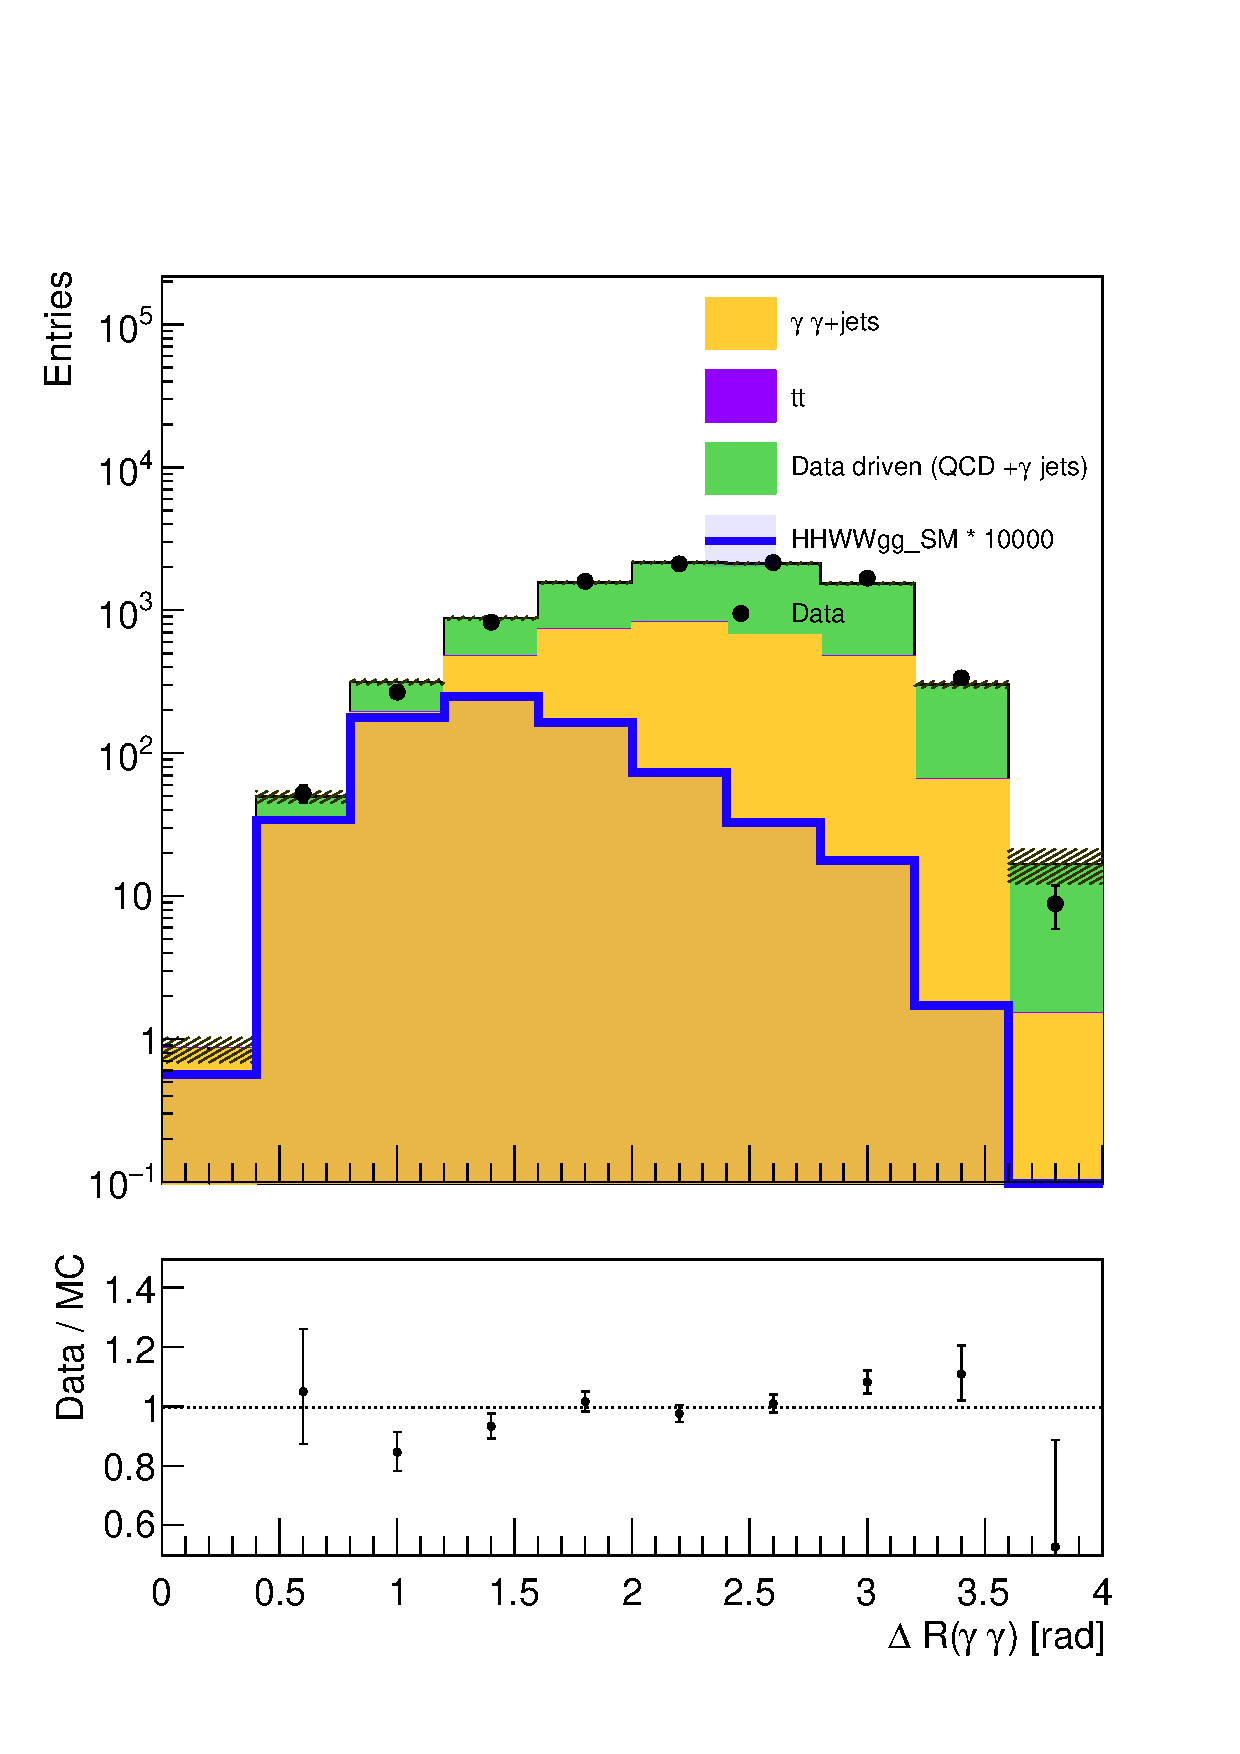
\includegraphics[width=0.45\textwidth]{Sections/HHWWgg/images/FH_DNN/DataMC/DataMC_New_DR_gg_SB_log.pdf}%
  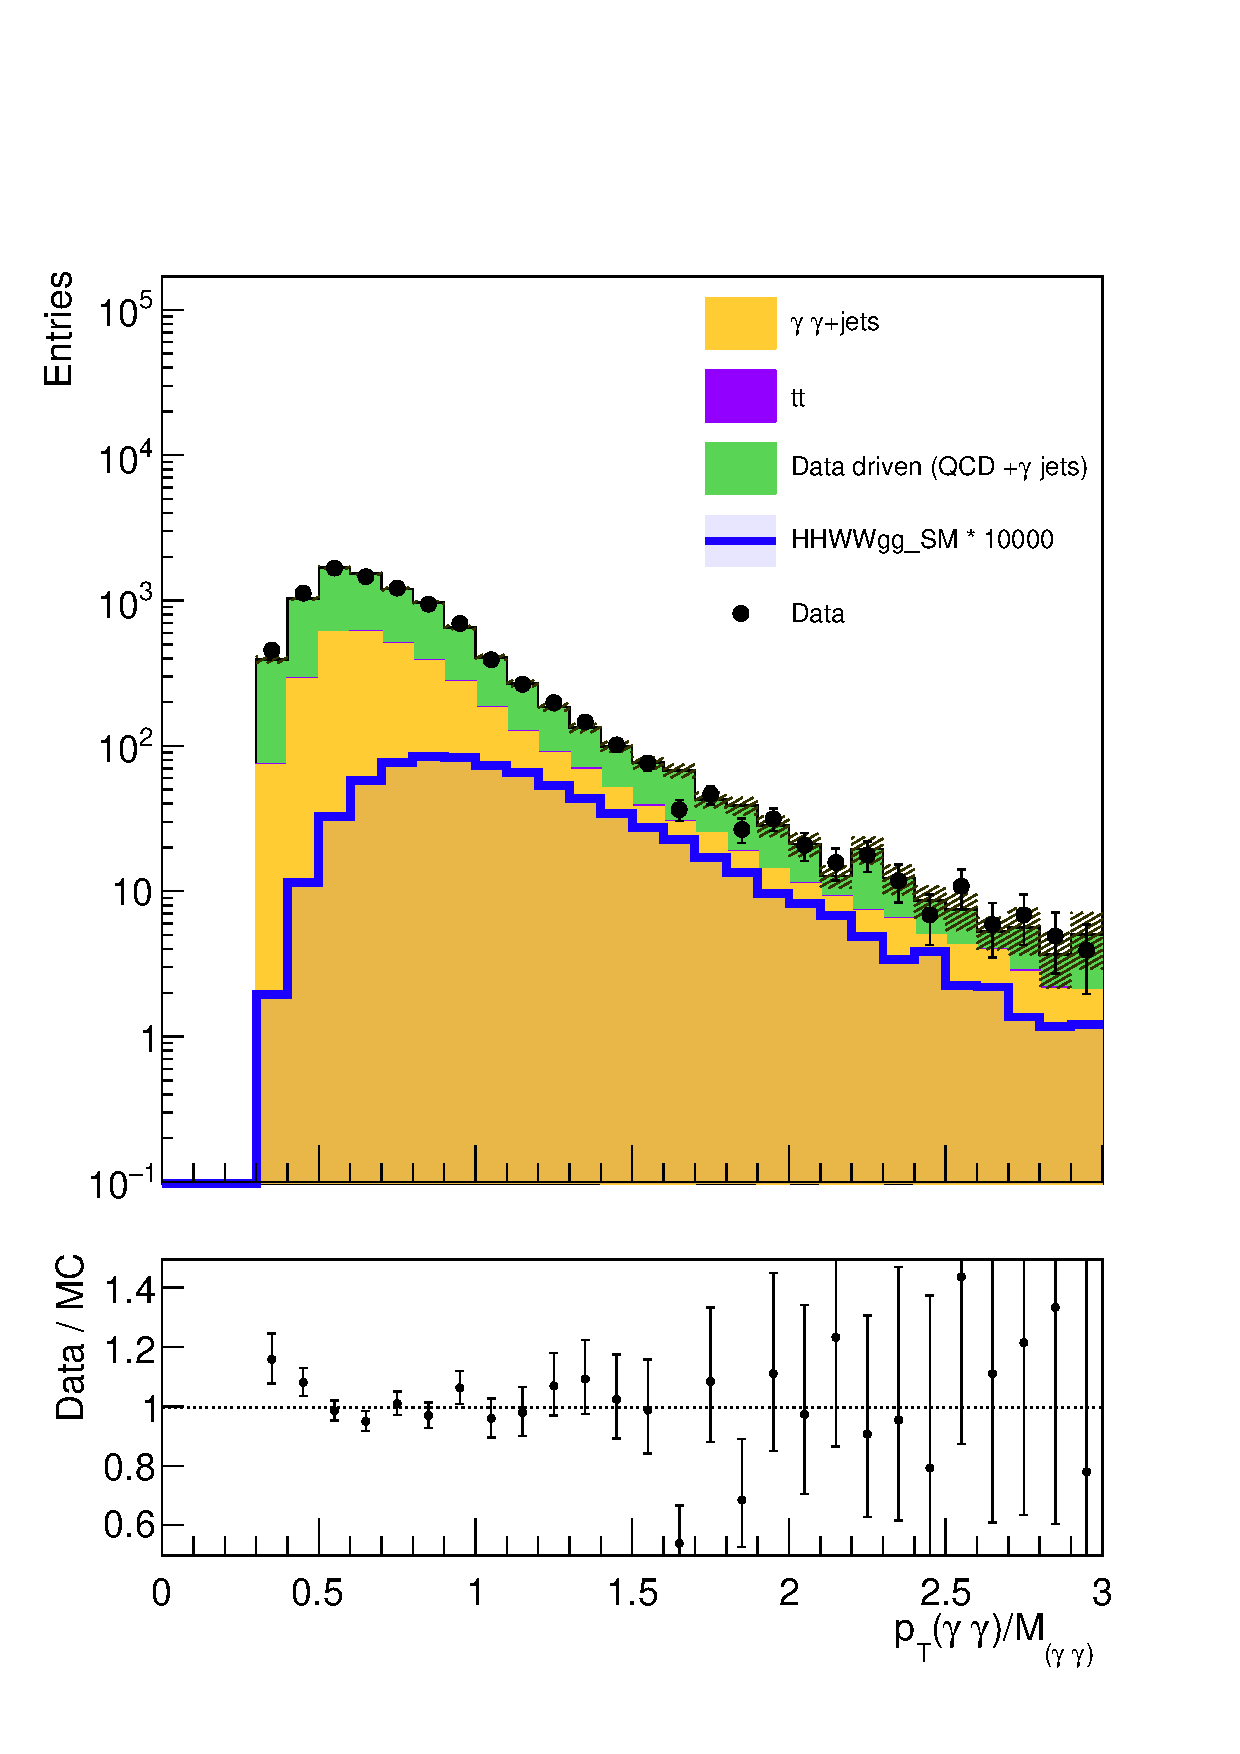
\includegraphics[width=0.45\textwidth]{Sections/HHWWgg/images/FH_DNN/DataMC/DataMC_Scaled_Leading_Photon_pt_SB_log.pdf}%
  \caption{Data/MC comparison of a fully-hadronic leading DNN input feature (left) and second leading DNN input feature (right).}
\label{fig:FH_DataMC_1}
\end{figure}

\begin{figure}[!htbp]
  \centering
  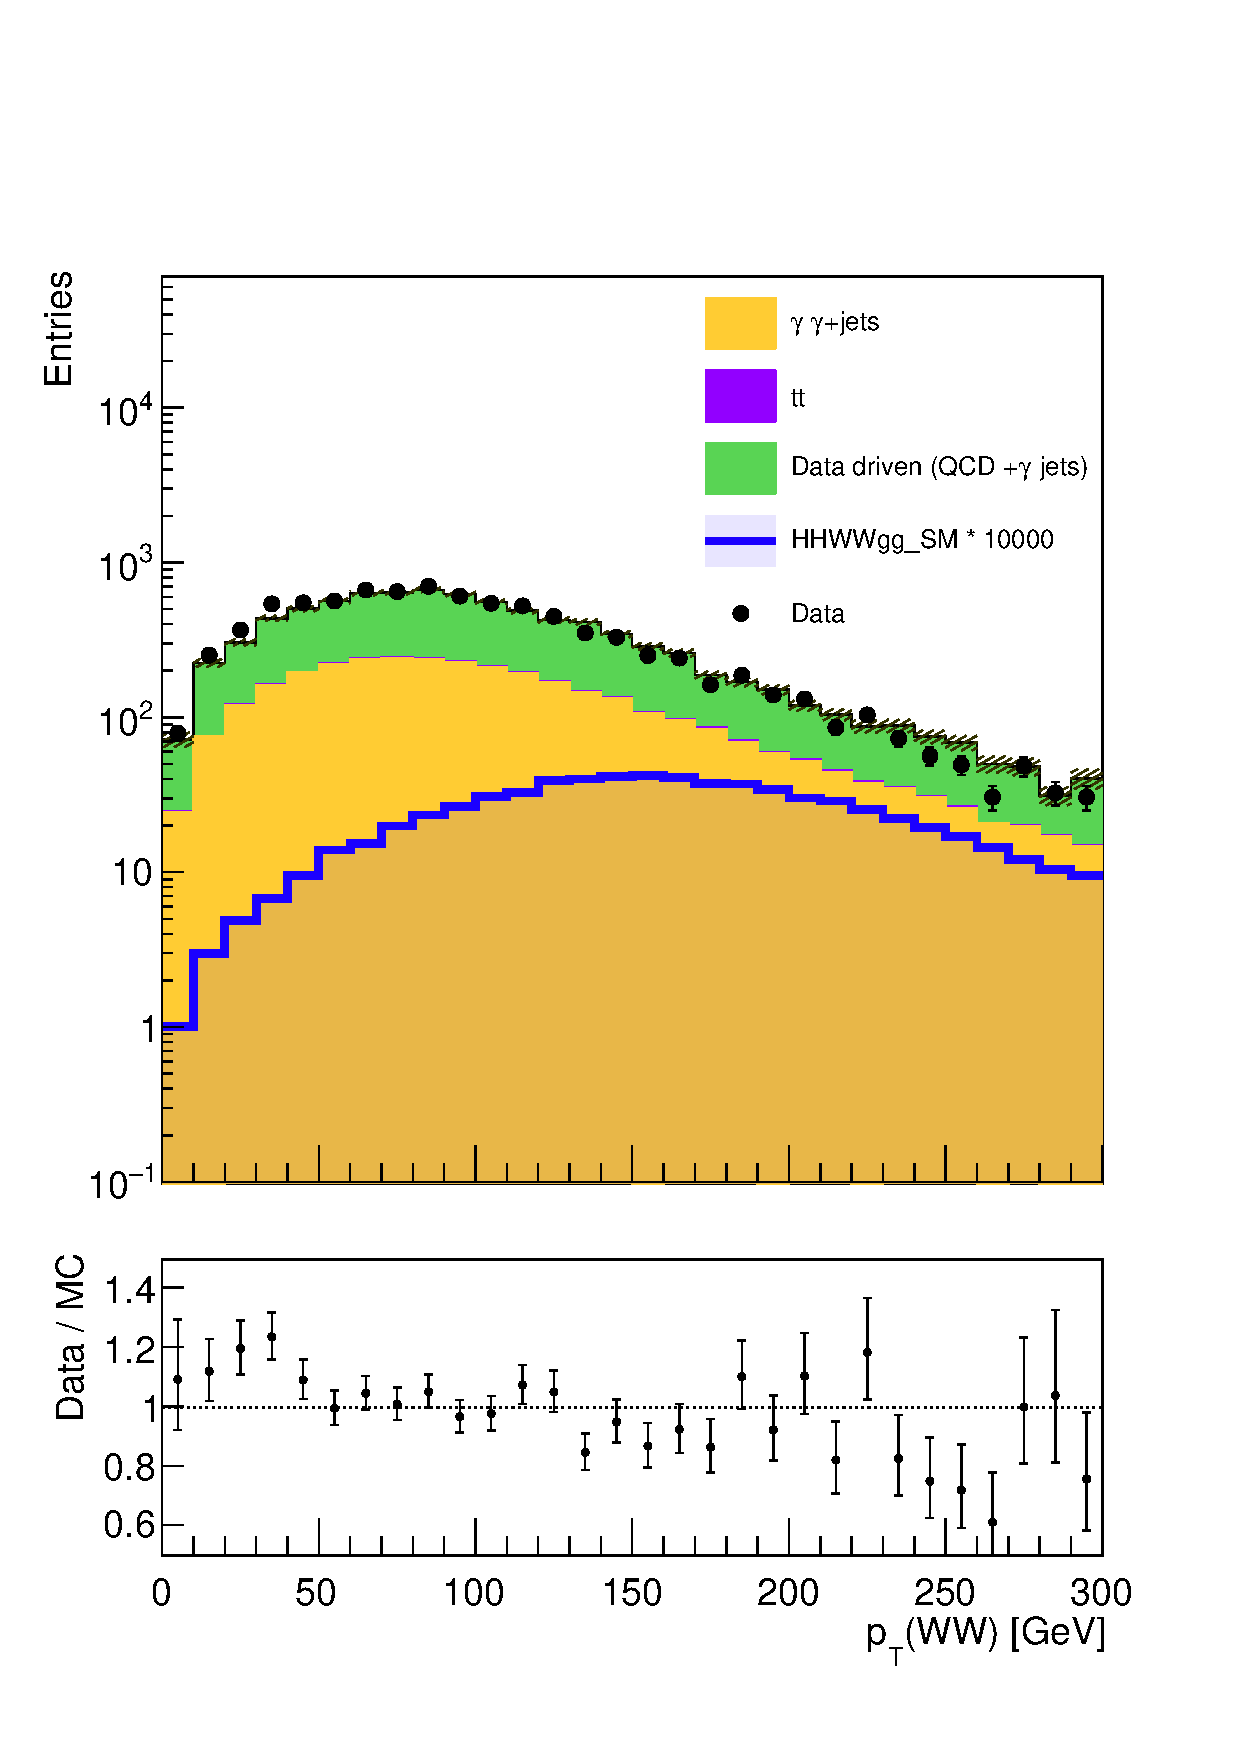
\includegraphics[width=0.45\textwidth]{Sections/HHWWgg/images/FH_DNN/DataMC/DataMC_New_pTBasedSel_WW_pT_SB_log.pdf}%
  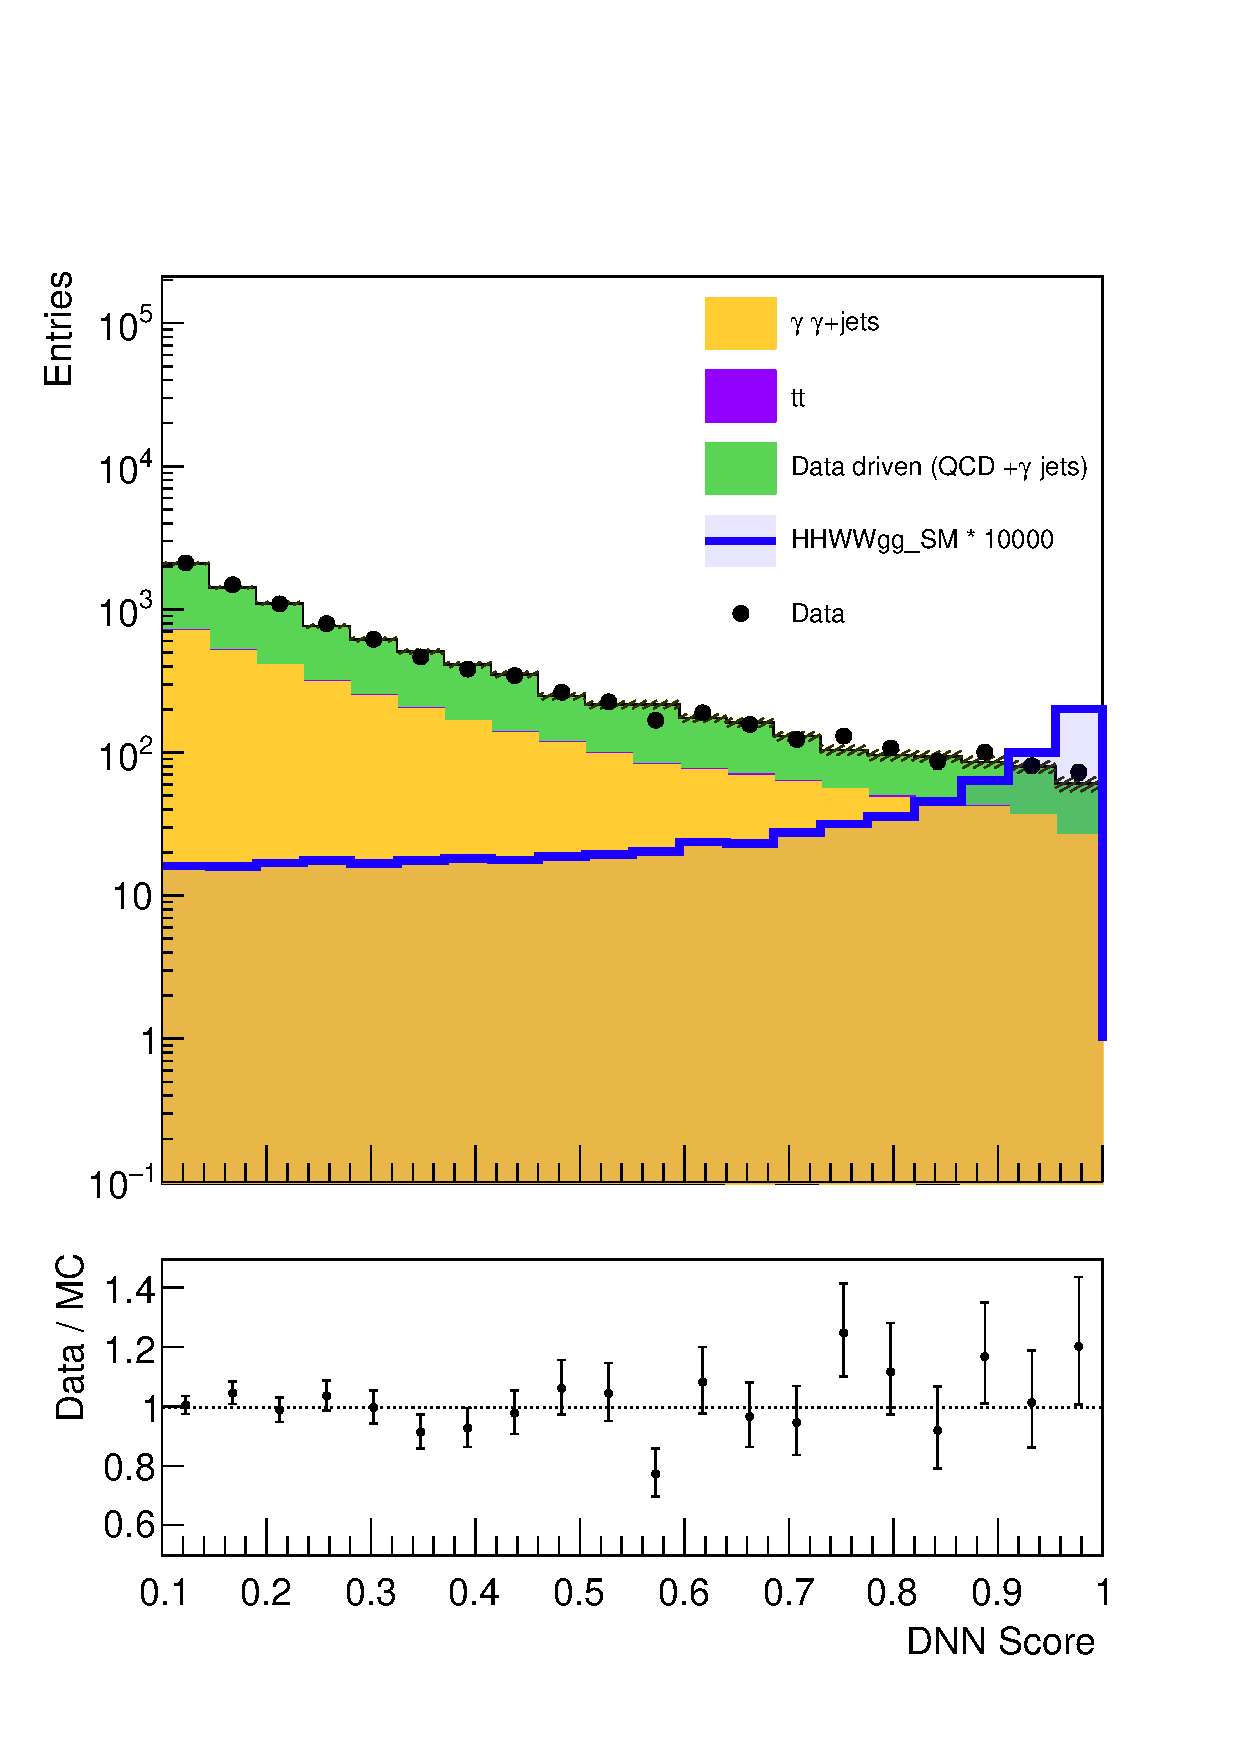
\includegraphics[width=0.45\textwidth]{Sections/HHWWgg/images/FH_DNN/DataMC/DataMC_evalDNN_WWvsAll_SB_log.pdf}%
  \caption{Data/MC comparison of a fully-hadronic third leading DNN input feature and DNN score.}
\label{fig:FH_DataMC_2}
\end{figure}


% The correlation between all input features is checked and shown in Fig.~\ref{fig:FH_DNN_CorrelationPlot}. For some of input features there are large correlations but for DNN it should not affect the result. So, variables having large correlations are not removed.

% \begin{figure}[!htbp]
%   \centering 
%   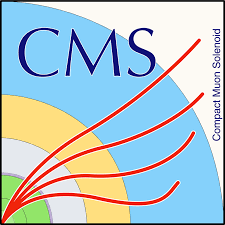
\includegraphics[width=0.5\textwidth]{Images/Logos/CMS_Logo.png}
% %   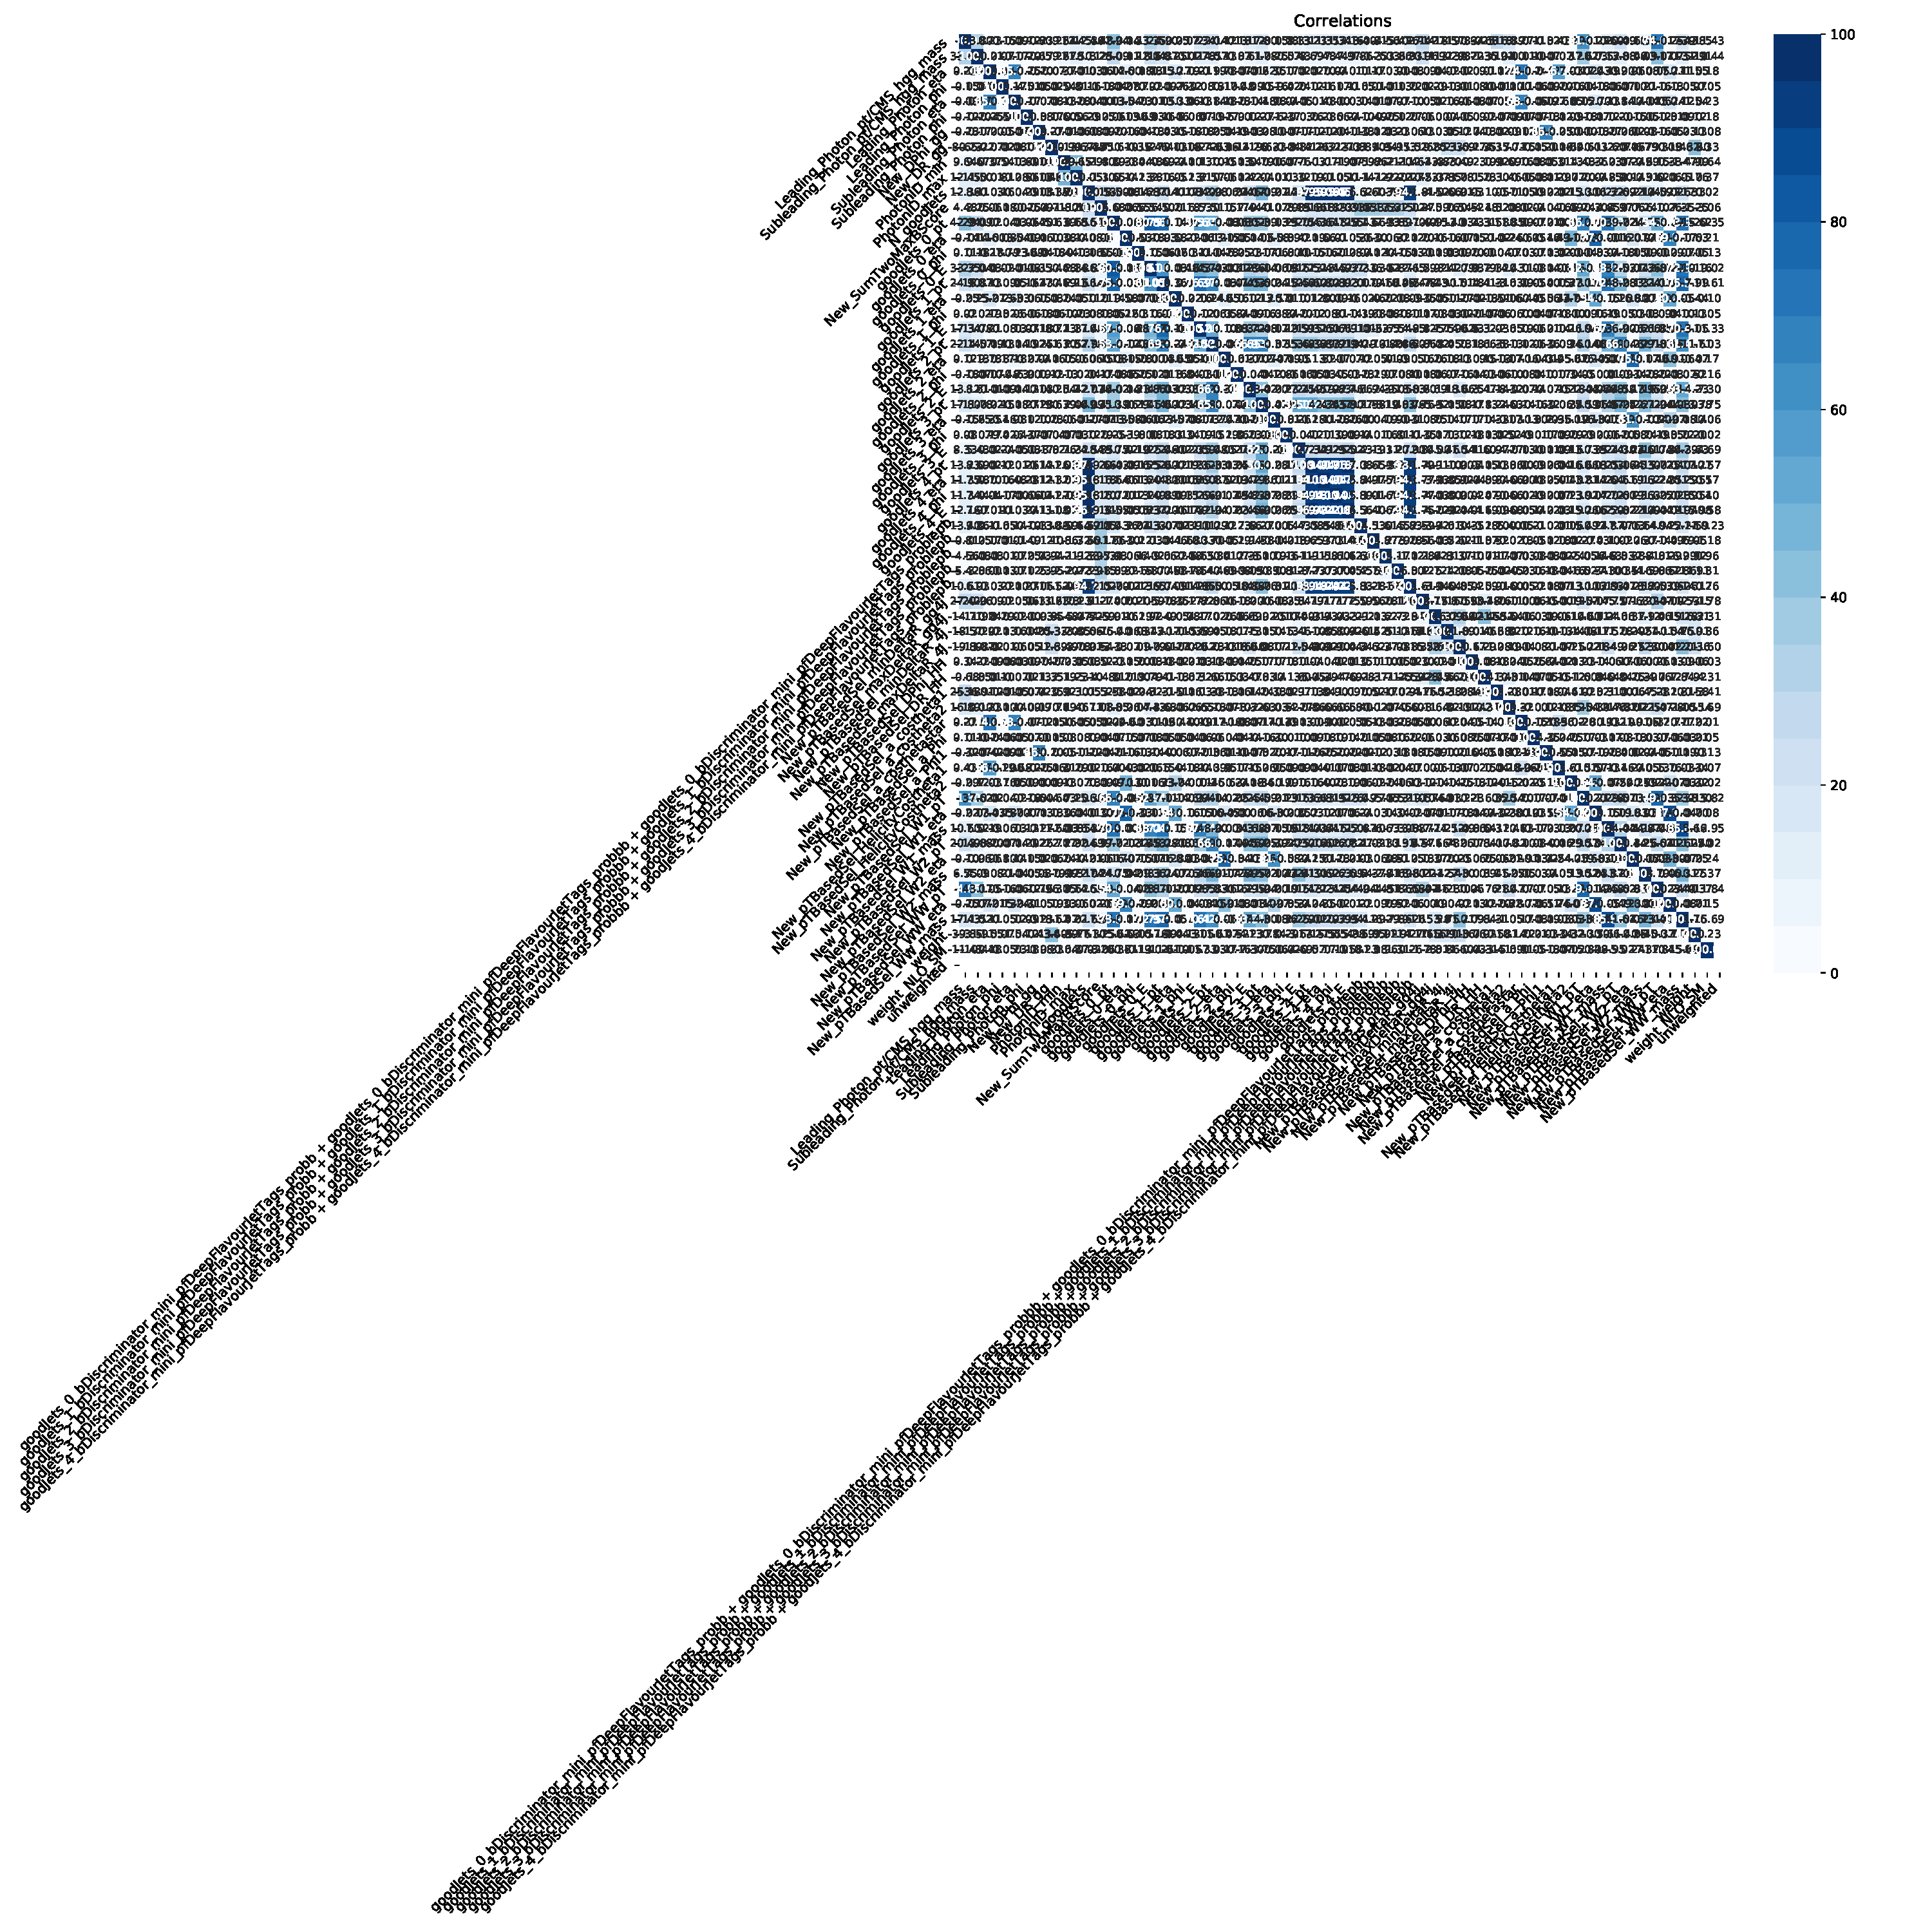
\includegraphics[width=\textwidth,trim={17cm 17cm 0 0},clip=true]{Sections/HHWWgg/images/FH_DNN/WWgg/correlation_plot.pdf}  
%   \caption{Correlation of Fully-Hadronic DNN WW$\gamma \gamma$ identifier training input features}
%   \label{fig:FH_DNN_CorrelationPlot}
% \end{figure}

% The DNN network optimized hyperparameter setting can be found in Tab.~\ref{tab:FH_DNN_HyperparameterSettings} and the one of best architecture that we investigated for the Fully-Hadronic channel, can be found in Fig.~\ref{fig:FH_DNN_Architecture}.
% \begin{table}[!htbp]
% \centering
% \caption{Hyper-parameter settings for WW$\gamma \gamma$ identifier training for the Fully-Hadronic channel DNN}
% % \resizebox{\textwidth}{!}
% {
% \begin{tabular}{| l | l |}
% \hline
% Hyper-Parameter & Settings \\
% \hline
% Epoch & 170 \\
% Learning rate & $10^{-3}$ \\
% Batch size & 250 \\
% % Dropout rate & 0.1 \\
% Optimizer & Nadam \\
% Loss function & categorical crossentropy \\
% Kernel initialiser & glorot normal \\
% Hidden layer activation function & elu \\
% Output layer activation function & softmax \\ \hline
% \end{tabular}
% }
% \label{tab:FH_DNN_HyperparameterSettings}
% \end{table}

% \begin{figure}[!htbp]
%   \centering
%   \includegraphics[height=0.5\textwidth]{Sections/HHWWgg/images/FH_DNN/WWgg/model_schematic.png}
%   % \includegraphics[height=0.5\textwidth,trim={0 30cm 0 0},clip=true]{Sections/HHWWgg/images/FH_DNNmodel_schematic.png}%
%   % \includegraphics[height=0.5\textwidth,trim={0 0 0 35cm},clip=true]{Sections/HHWWgg/images/FH_DNNmodel_schematic.png}
%   \caption{DNN network architecture. This architecture is used by both training - a) WW$\gamma \gamma$ identifier, and b) bb$\gamma \gamma$ killer.}
%   \label{fig:FH_DNN_Architecture}
% \end{figure}
% \begin{figure}[!htbp]
%   \centering
%   \includegraphics[height=\textheight]{Sections/HHWWgg/images/FH_DNNmodel_schematic.png}%
%   \caption{Correlation of Fully-Hadronic DNN input features}
%   \label{fig:FH_DNN_Architecture1}
% \end{figure}

The output ROC curve from the training is shown in Fig.~\ref{fig:FH_DNN_ROC}.

% and couple of other metrics are shown in Fig.~\ref{fig:FH_DNN_Metrics}. 

As the curves are similar, this indicates no sign of over-training. Additionally, the output score of signal and background for training and testing shows no overtraining signature, as shown in Fig.~\ref{fig:FH_DNN_OutputScore}.

In addition, a check is performed in a dedicated control region to demonstrate that a large difference in data and MC acceptance is not expected to be introduced by the
WW$\gamma\gamma$ identifier DNN, and that the DNN behaves as expected on its signal topology. This check is shown in Appendix \ref{sec:DNN_and_signal_validation}.

\begin{figure}[!htbp]7
  \centering
  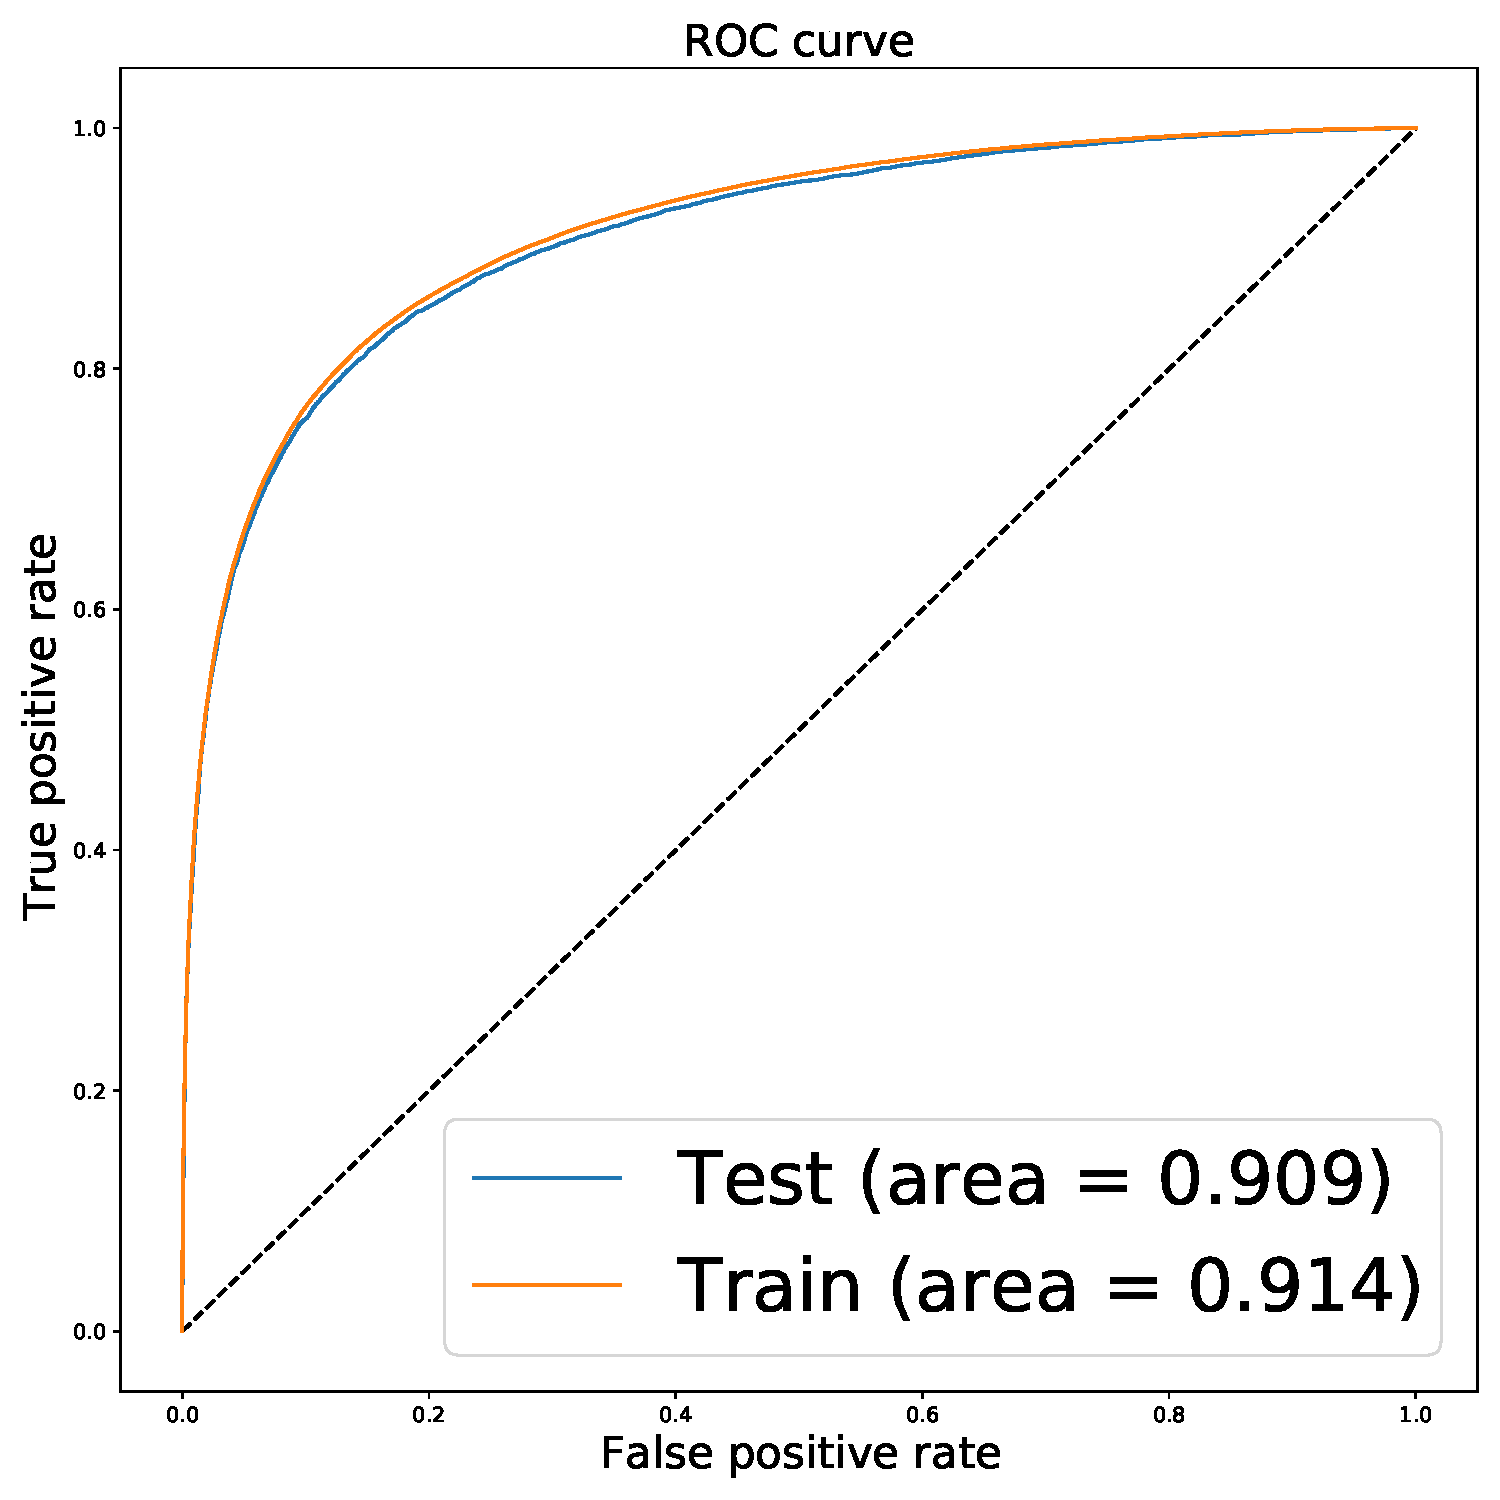
\includegraphics[scale=0.4]{Sections/HHWWgg/images/FH_DNN/WWgg/ROC.pdf}%
  \caption{ROC curve for WW$\gamma\gamma$ identifier Fully-Hadronic DNN}
  \label{fig:FH_DNN_ROC}
\end{figure}

% \begin{figure}[!htbp]
%   \centering
%   % \includegraphics[width=0.7\textwidth]{Sections/HHWWgg/images/FH_DNNall_metrics_nomgg.pdf}%
%   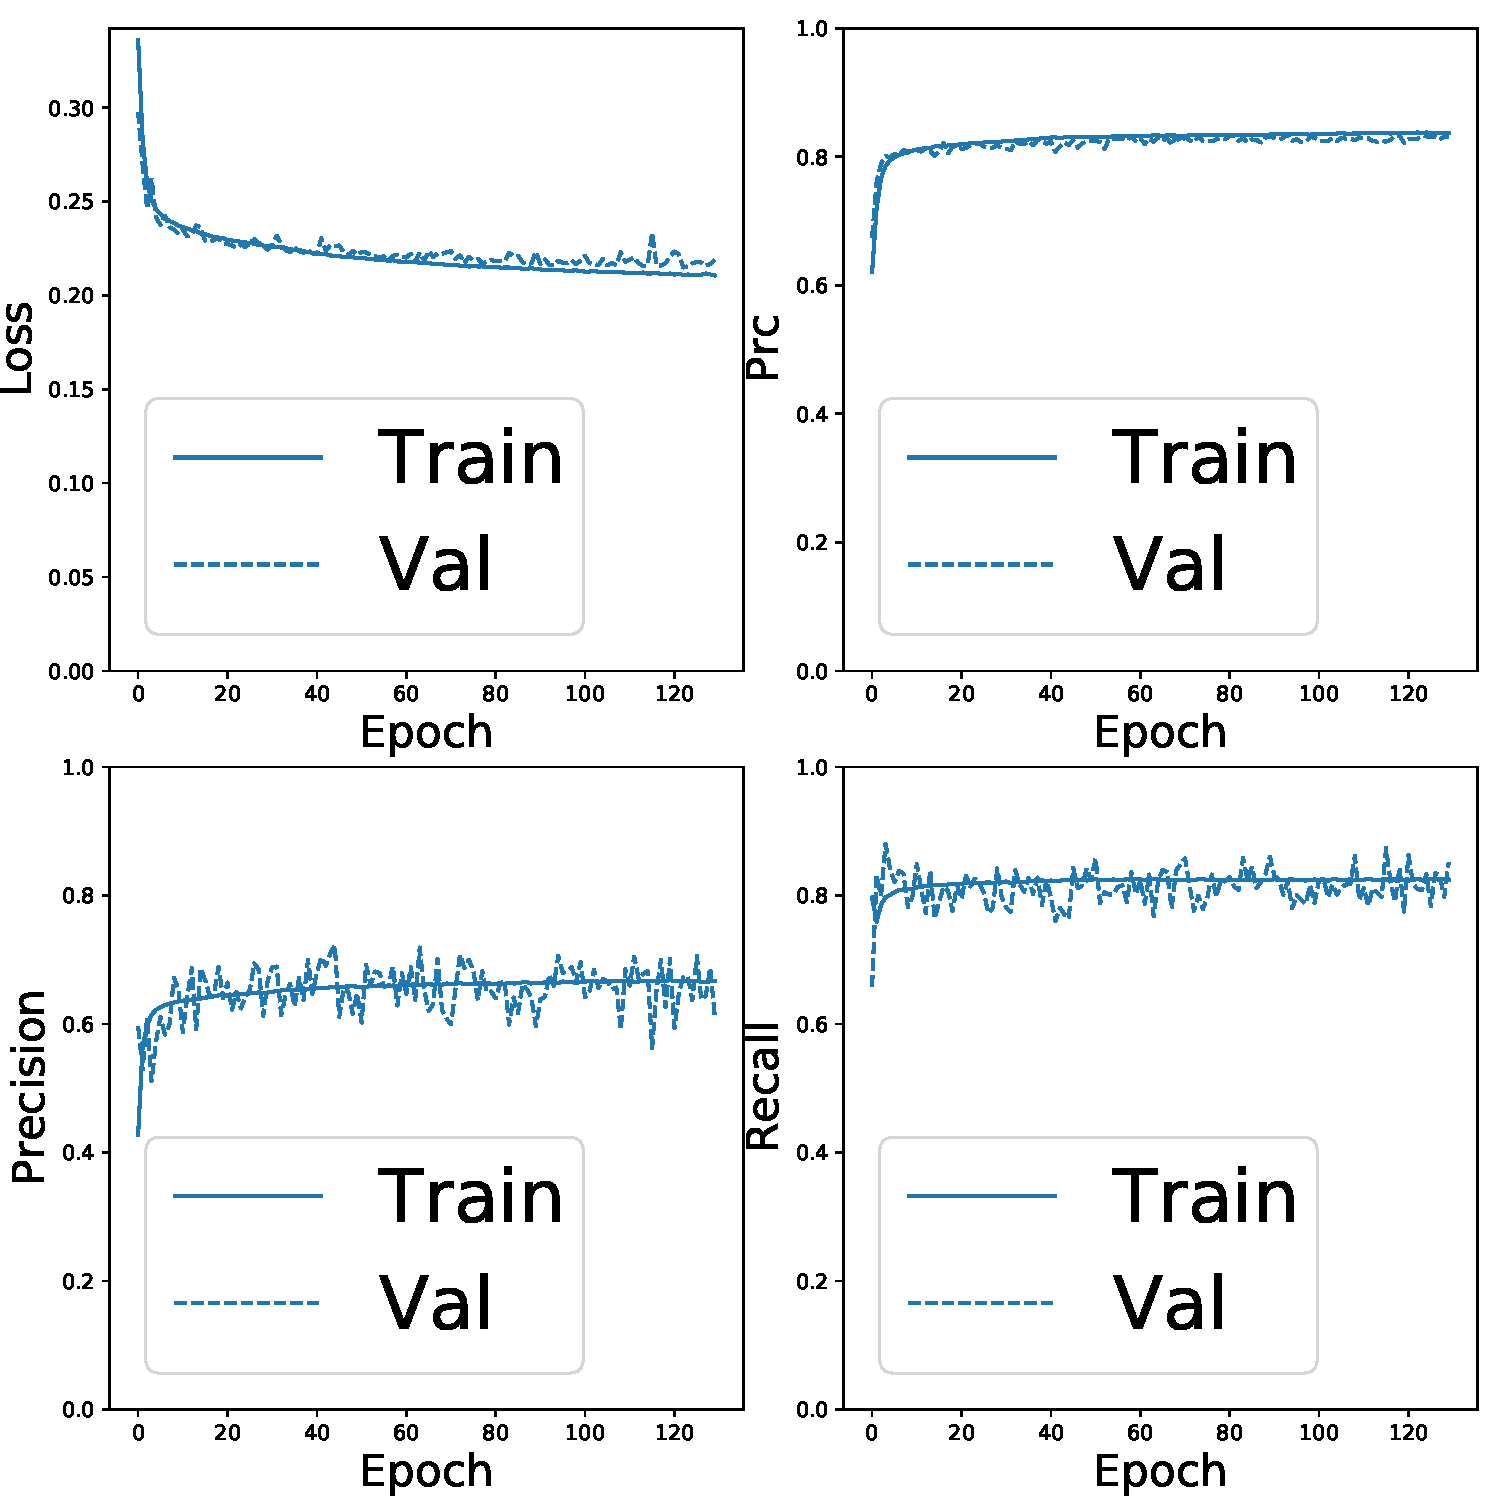
\includegraphics[scale=0.4]{Sections/HHWWgg/images/FH_DNN/WWgg/all_metrics.pdf}%
%   \caption{Metrics for Fully-Hadronic DNN WW$\gamma \gamma$ identifier. Loss w.r.t. epoch(top left). Precision-Recall curve w.r.t. epoch. Precision is defined as $\frac{(TruePositive)}{(TruePositive)+(FalsePositive)}$ and recall is defined as $\frac{(TruePositive)}{(TruePositive)+(FalseNegative)}$(top right). Precision w.r.t. epoch (bottom left). Recall w.r.t. epoch (bottom right).}
%   \label{fig:FH_DNN_Metrics}
% \end{figure}

\begin{figure}[!htbp]
  \centering
  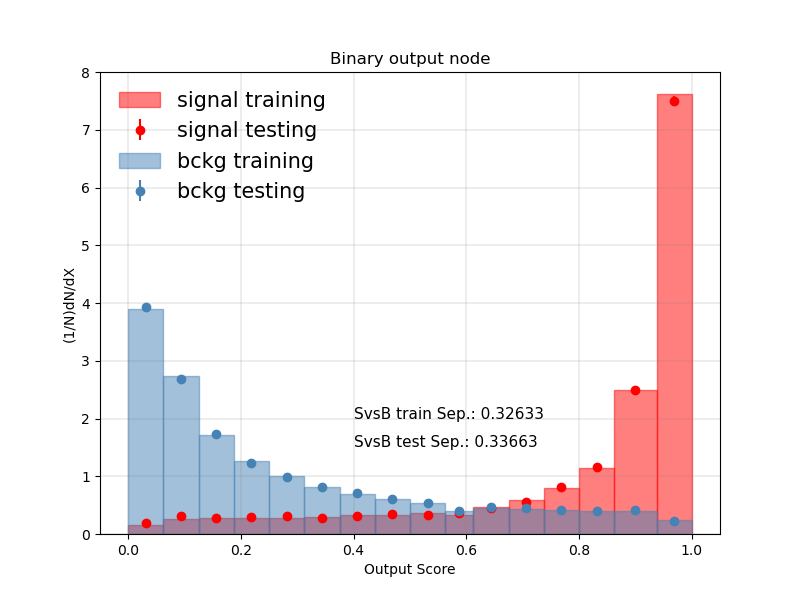
\includegraphics[scale=0.6]{Sections/HHWWgg/images/FH_DNN/WWgg/overfitting_plot_BinaryClassifier_Binary.png}%
  \caption{Output score of Fully-Hadronic DNN WW$\gamma \gamma$ identifier training}
  \label{fig:FH_DNN_OutputScore}
\end{figure}

\subsubsection{bb$\gamma\gamma$ killer}

This binary DNN training is used as a bb$\gamma\gamma$ killer. The objective of this DNN is to output a bb$\gamma\gamma$ killer score to use as a discriminant to use for the removal of bb$\gamma\gamma$ events from the WW$\gamma\gamma$ phase-space. This is trained considering a bb$\gamma\gamma$ simulation sample as signal. The list of background used consists of all background mentioned in Tab.~\ref{tab:fullyHadronicMCBkg} along with the Fully-hadronic WW$\gamma\gamma$ simulation sample. Other details for this training including the events selections, list of input variables and DNN architecture remain the same as for the WW$\gamma\gamma$ identifier described in Section \ref{subsubsec:FullyHadronicDNN}. 

% The correlation between all the input features are checked and shown in Fig.~\ref{fig:FH_DNN_CorrelationPlot_bbggVsAll}. For some of input features there are large correlations but for DNN it should not affect the result. So, variables having large correlations are not removed.
% \begin{figure}[!htbp]
%   \centering 
%   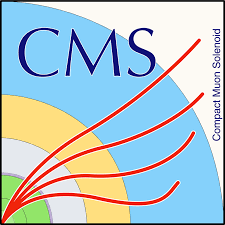
\includegraphics[width=0.5\textwidth]{Images/Logos/CMS_Logo.png}
% %   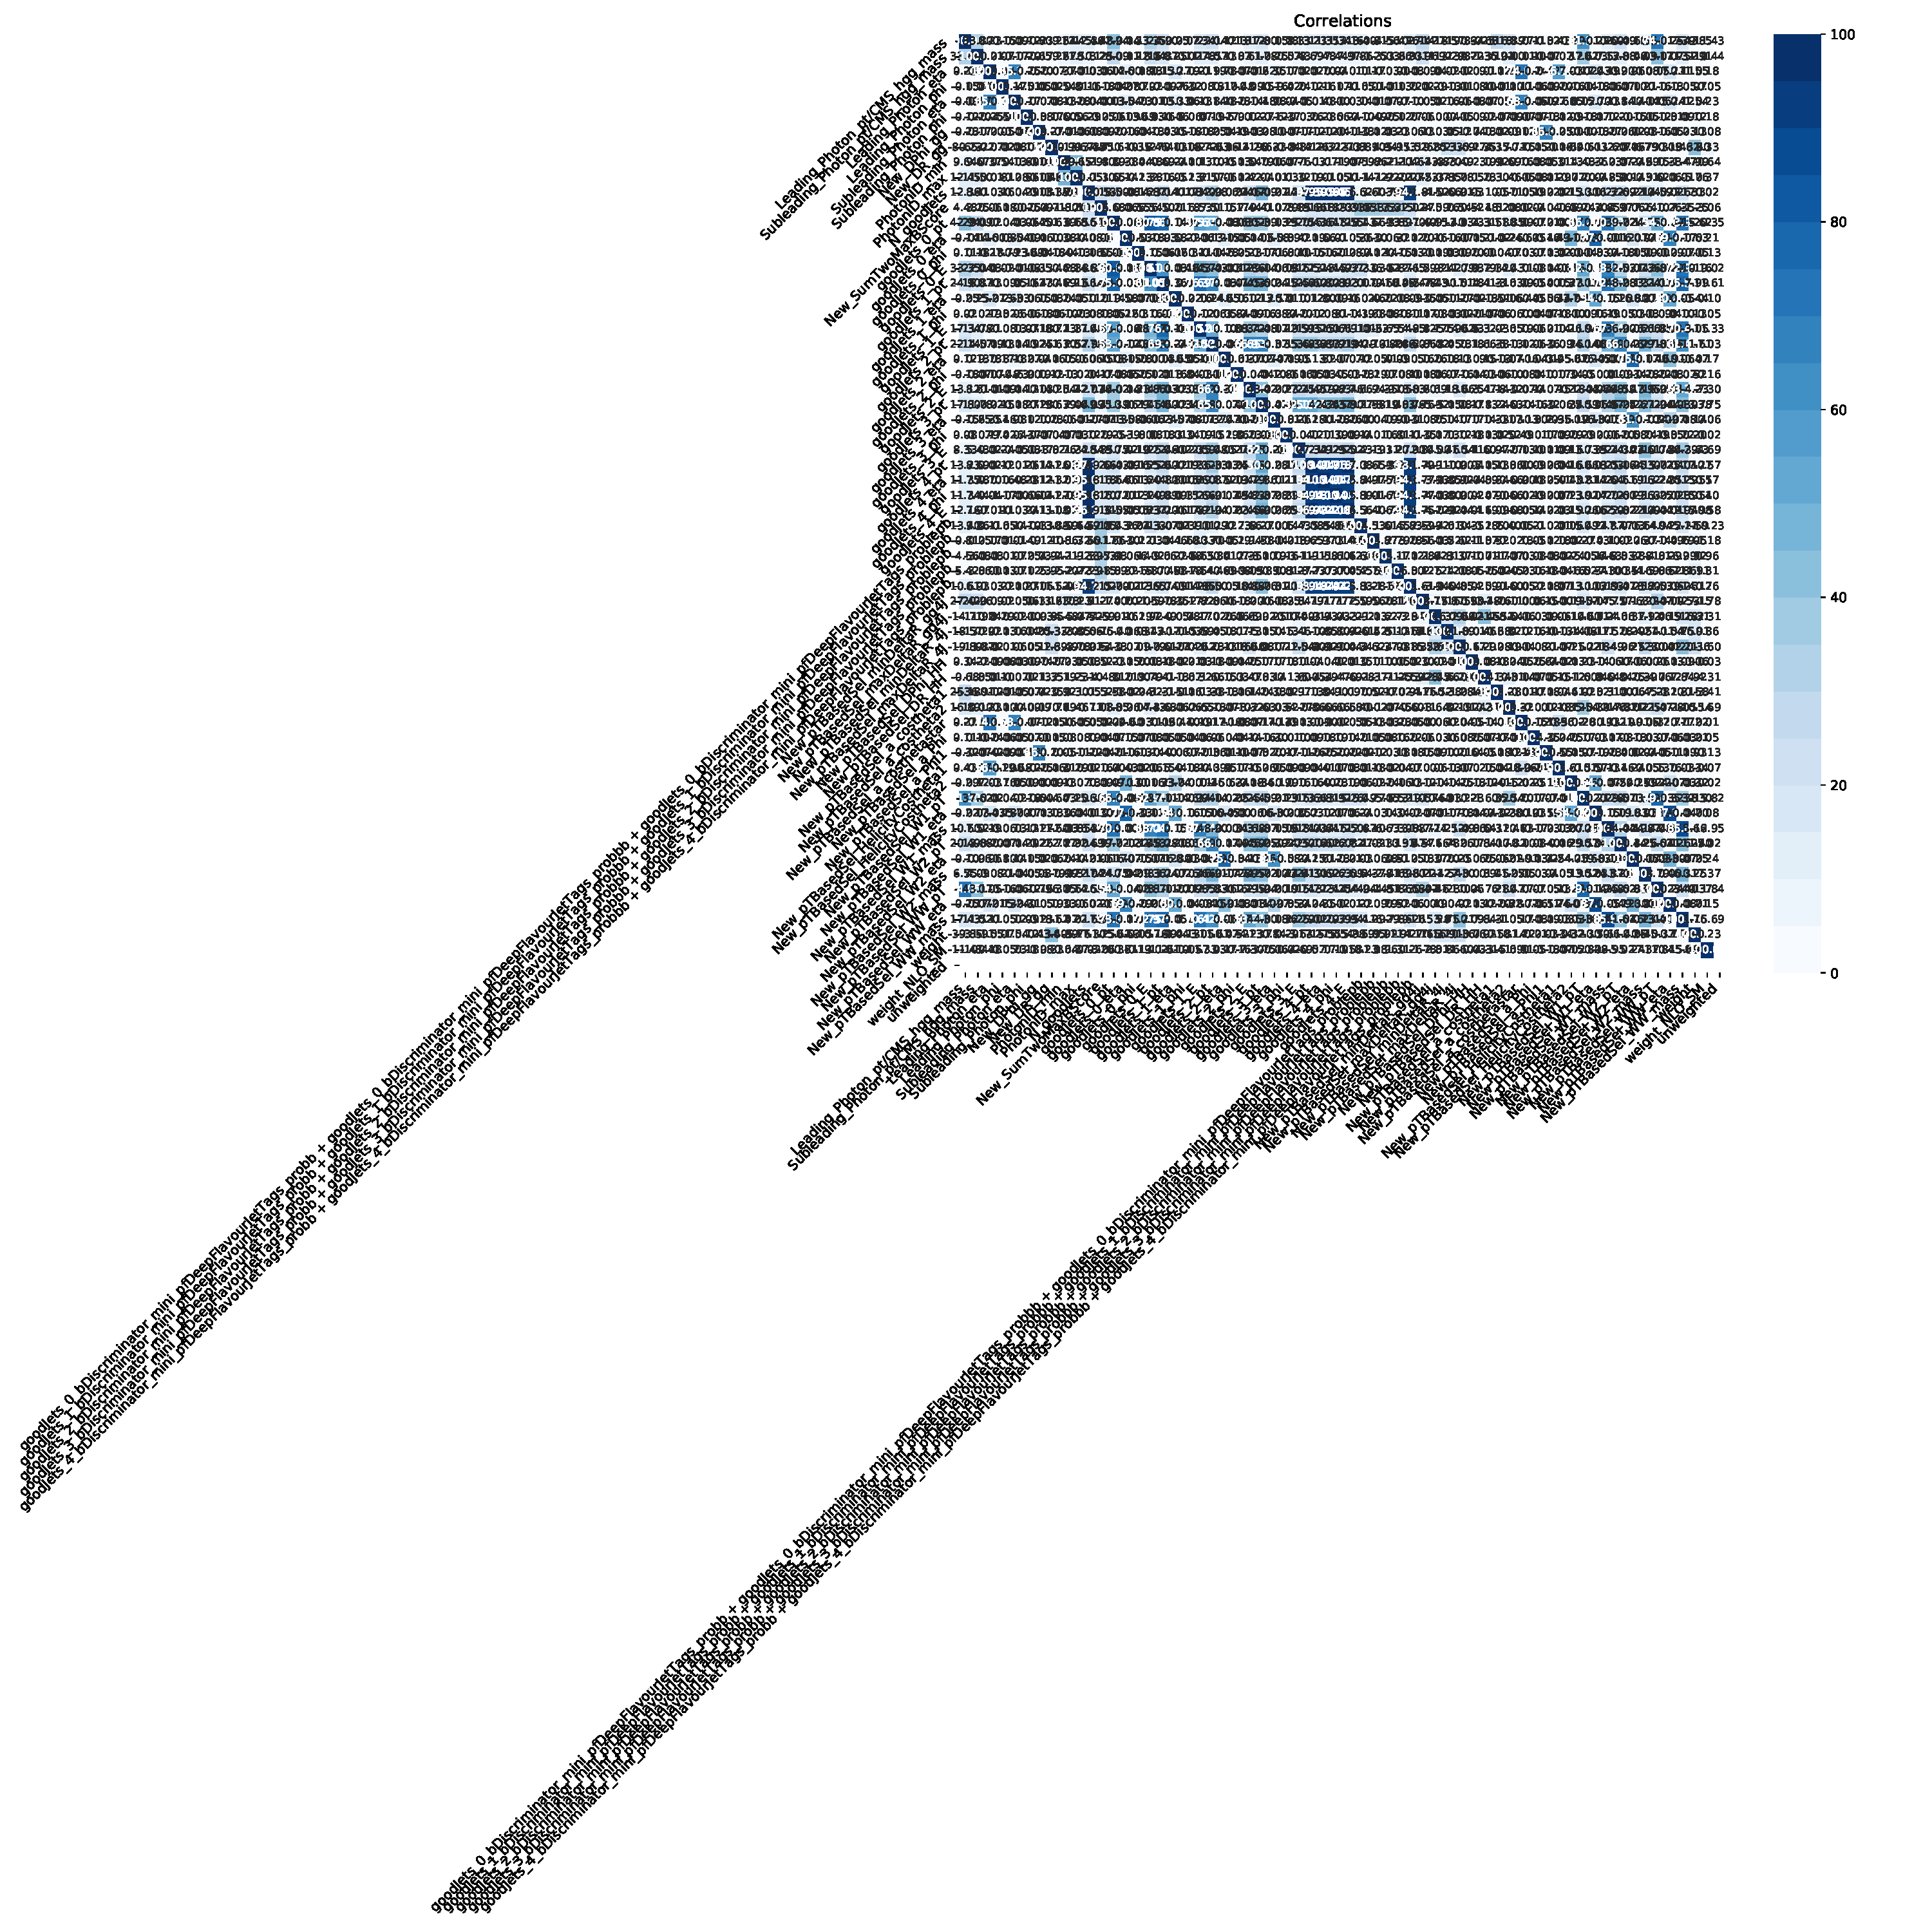
\includegraphics[width=\textwidth,trim={17cm 17cm 0 0},clip=true]{Sections/HHWWgg/images/FH_DNN/WWgg/correlation_plot.pdf}  
% %   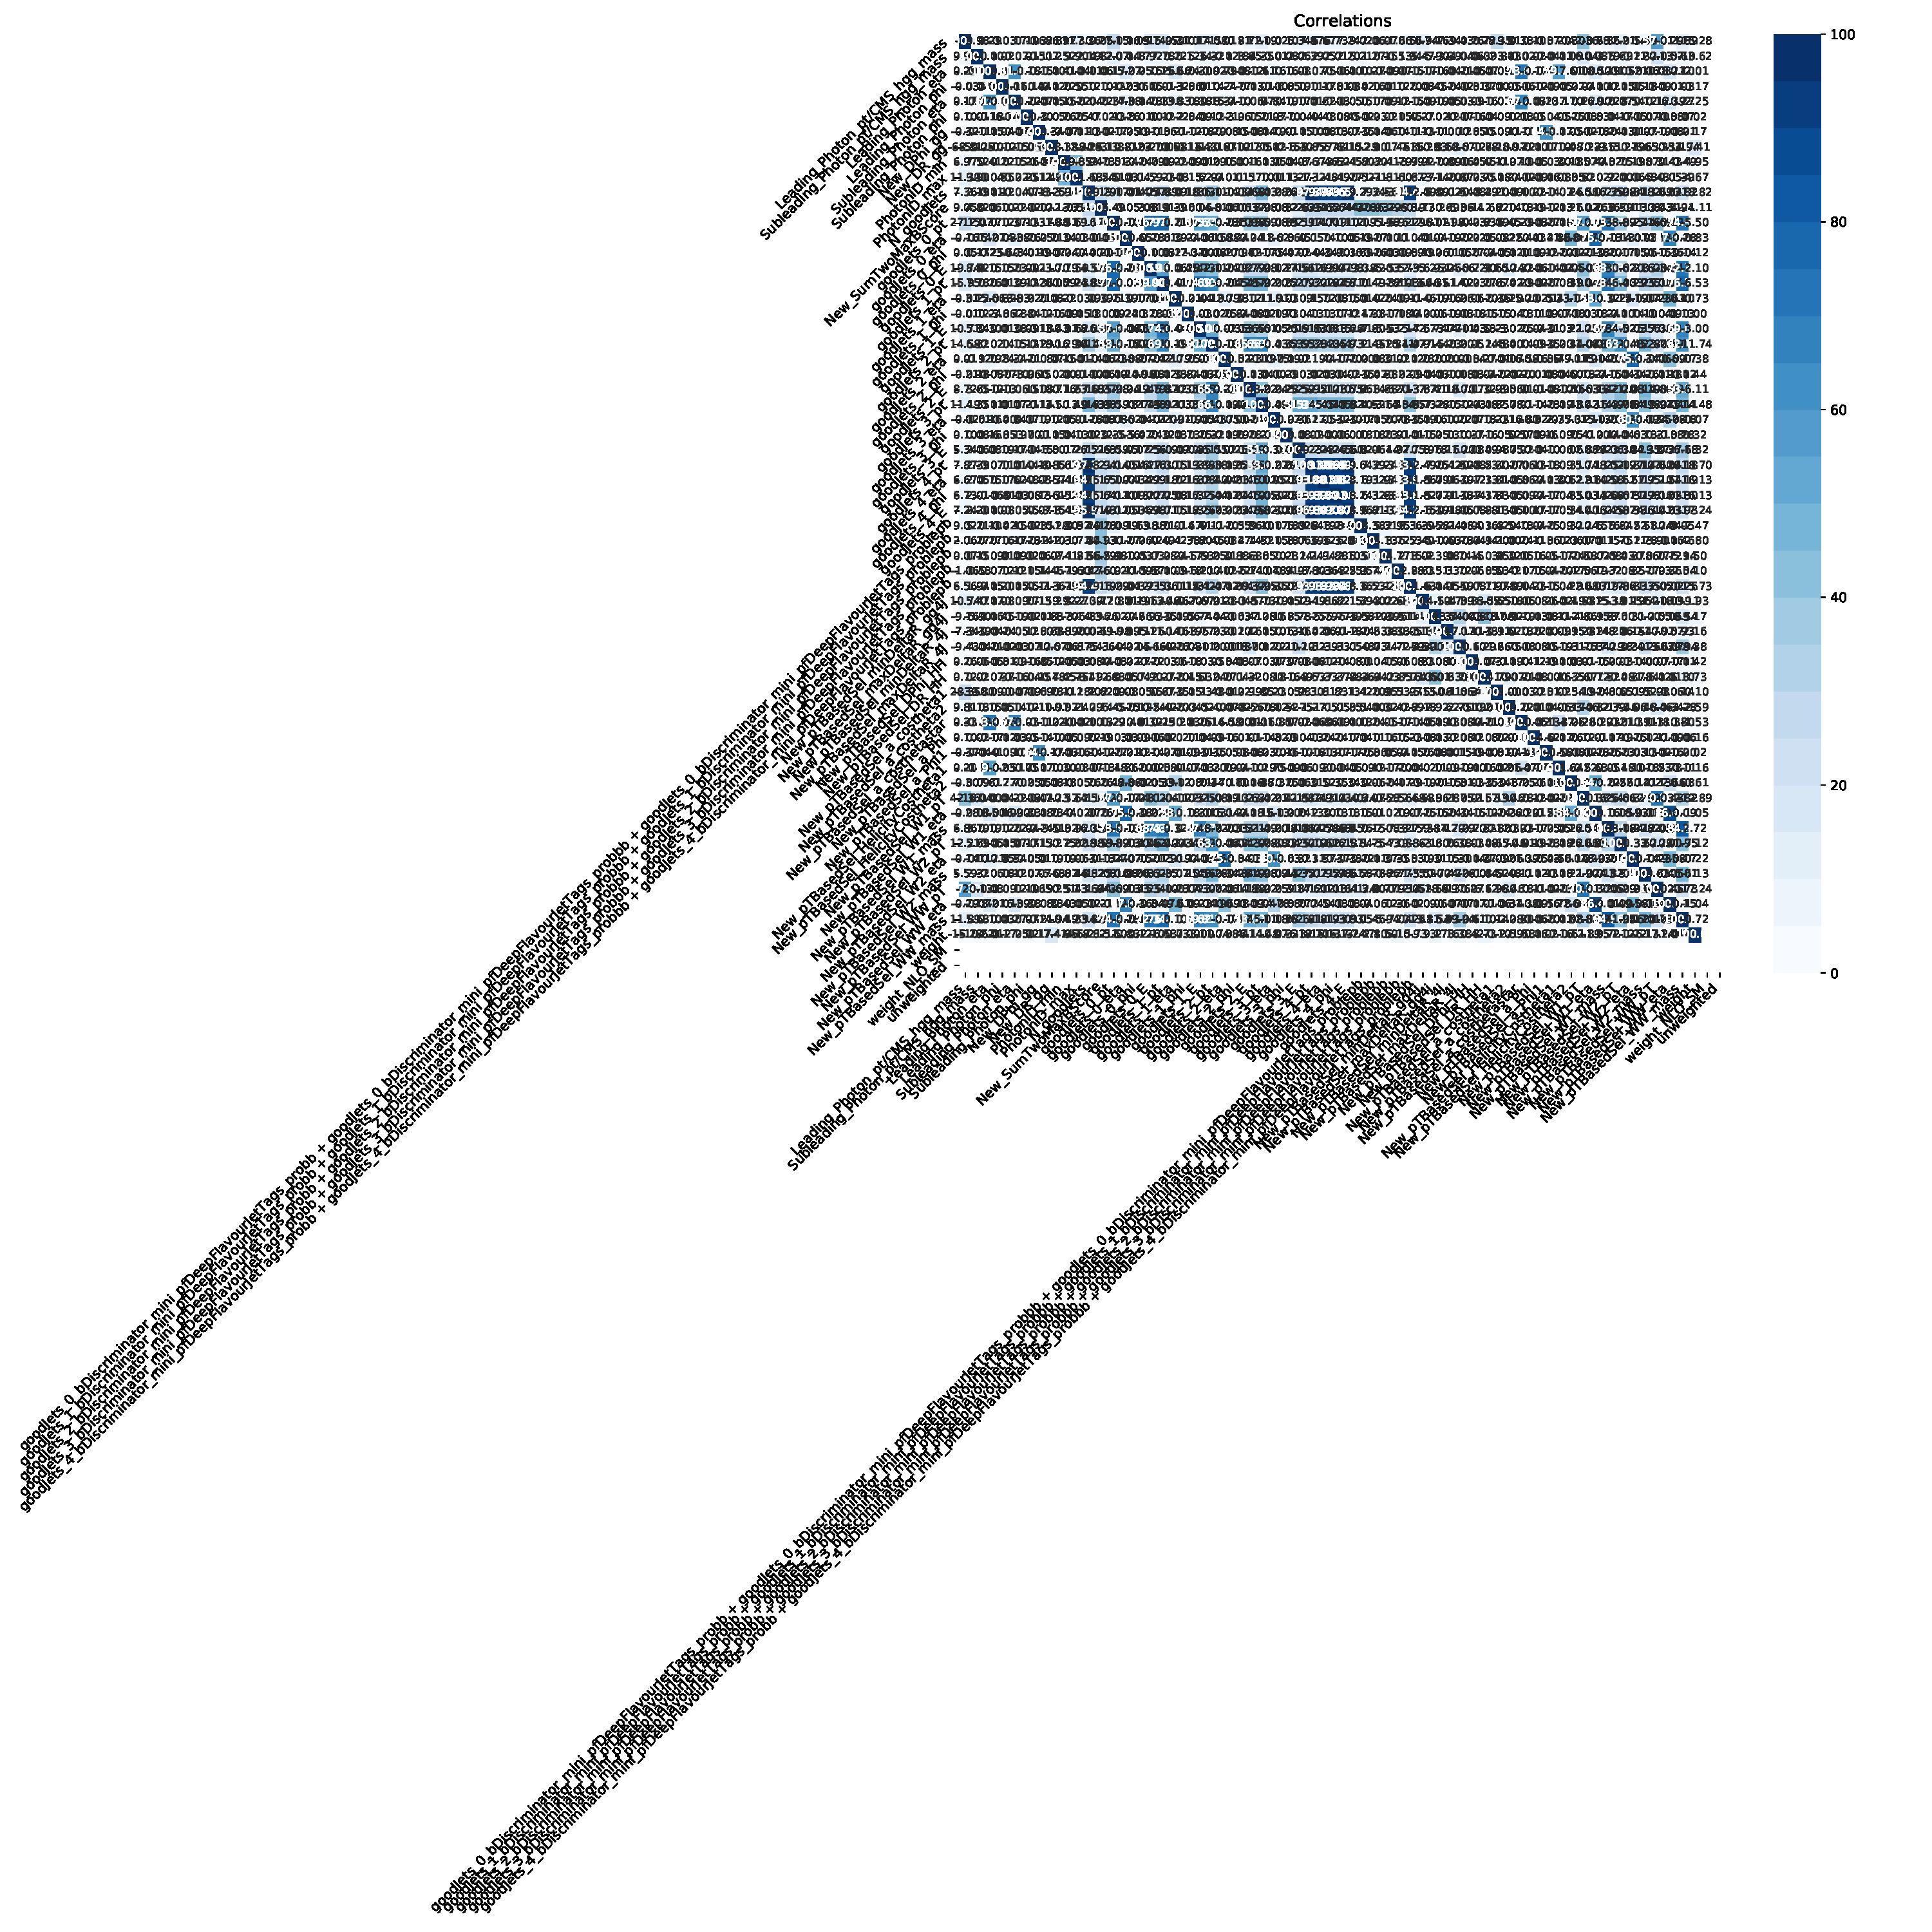
\includegraphics[width=\textwidth,trim={17cm 17cm 0 0},clip=true]{Sections/HHWWgg/images/FH_DNN/BBgg/correlation_plot.pdf}
%   \caption{Correlation of Fully-Hadronic DNN bb$\gamma \gamma$ killer input features}
%   \label{fig:FH_DNN_CorrelationPlot_bbggVsAll}
% \end{figure}

% The DNN network optimized hyperparameter setting can be found in Tab.~\ref{tab:FH_DNN_HyperparameterSettings_bbggVsAll} and the one of best architecture that we investigated is same as used in Training -1, i.e. Fig.~\ref{fig:FH_DNN_Architecture}.
% \begin{table}[!htbp]
% \centering
% \caption{Hyper-parameter settings for bb$\gamma \gamma$ killer training for Fully-Hadronic channel}
% % \resizebox{\textwidth}{!}
% {
% \begin{tabular}{| l | l |}
% \hline
% Hyper-Parameter & Settings \\
% \hline
% Epoch & 400 \\
% Learning rate & $10^{-4}$ \\
% Batch size & 150 \\
% % Dropout rate & 0.1 \\
% Optimizer & Adam \\
% Loss function & categorical crossentropy \\
% Kernel initialiser & glorot normal \\
% Hidden layer activation function & elu \\
% Output layer activation function & softmax \\ \hline
% \end{tabular}
% }
% \label{tab:FH_DNN_HyperparameterSettings_bbggVsAll}
% \end{table}



% \begin{figure}[!htbp]
%   \centering
%   \includegraphics[height=0.5\textwidth]{Sections/HHWWgg/images/FH_DNN/BBgg/model_schematic.png}
%   % \includegraphics[height=0.5\textwidth,trim={0 30cm 0 0},clip=true]{Sections/HHWWgg/images/FH_DNN/BBgg/model_schematic.png}%
%   % \includegraphics[height=0.5\textwidth,trim={0 0 0 35cm},clip=true]{Sections/HHWWgg/images/FH_DNN/BBgg/model_schematic.png}
%   \caption{DNN network architecture}
%   \label{fig:FH_DNN_Architecture_bbggVsAll}
% \end{figure}
% \begin{figure}[!htbp]
%   \centering
%   \includegraphics[height=\textheight]{Sections/HHWWgg/images/FH_DNNmodel_schematic.png}%
%   \caption{Correlation of Fully-Hadronic DNN input features}
%   \label{fig:FH_DNN_Architecture1_bbggVsAll}
% \end{figure}

The output ROC curve of this training is shown in Fig.~\ref{fig:FH_DNN_ROC_bbggVsAll}. As the curves are similar for both the training and test datasets, this indicates that there is no overtraining. Additionally, the output score of signal and background for training and testing shows no overtraining signature,
as shown in Fig.~\ref{fig:FH_DNN_OutputScore_bbggVsAll}.

% and couple of other metrics are shown in Fig.~\ref{fig:FH_DNN_Metrics_bbggVsAll}.


% All of them shows no sign of over-training. Also, the output score of signal and background for training and testing shows no overtraining signature,
% as shown in Fig.~\ref{fig:FH_DNN_OutputScore_bbggVsAll}.

\begin{figure}[!htbp]
  \centering
  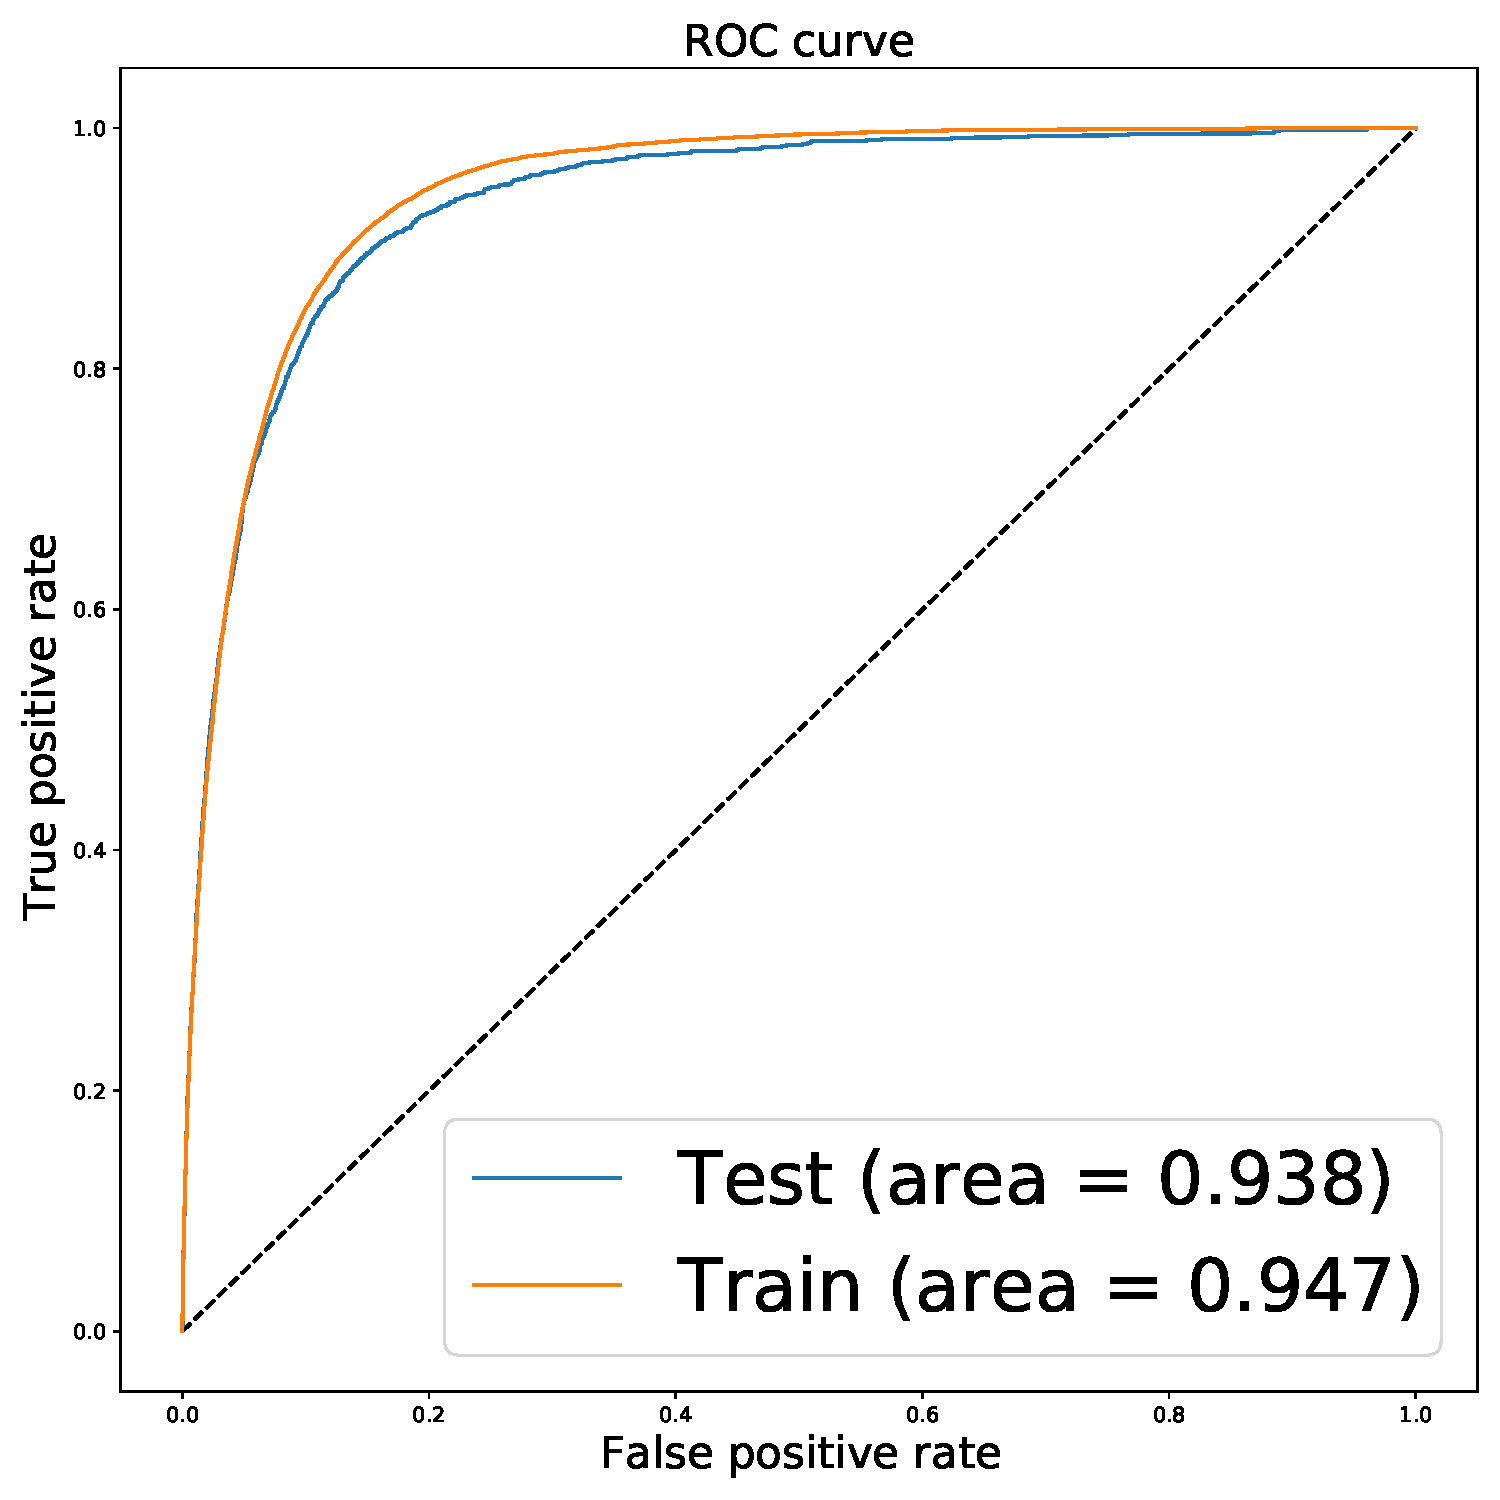
\includegraphics[scale=0.4]{Sections/HHWWgg/images/FH_DNN/BBgg/ROC.pdf}%
  \caption{ROC curve for Fully-Hadronic DNN bb$\gamma \gamma$ killer}
  \label{fig:FH_DNN_ROC_bbggVsAll}
\end{figure}

% \begin{figure}[!htbp]
%   \centering
%   % \includegraphics[width=0.7\textwidth]{Sections/HHWWgg/images/FH_DNNall_metrics_nomgg.pdf}%
%   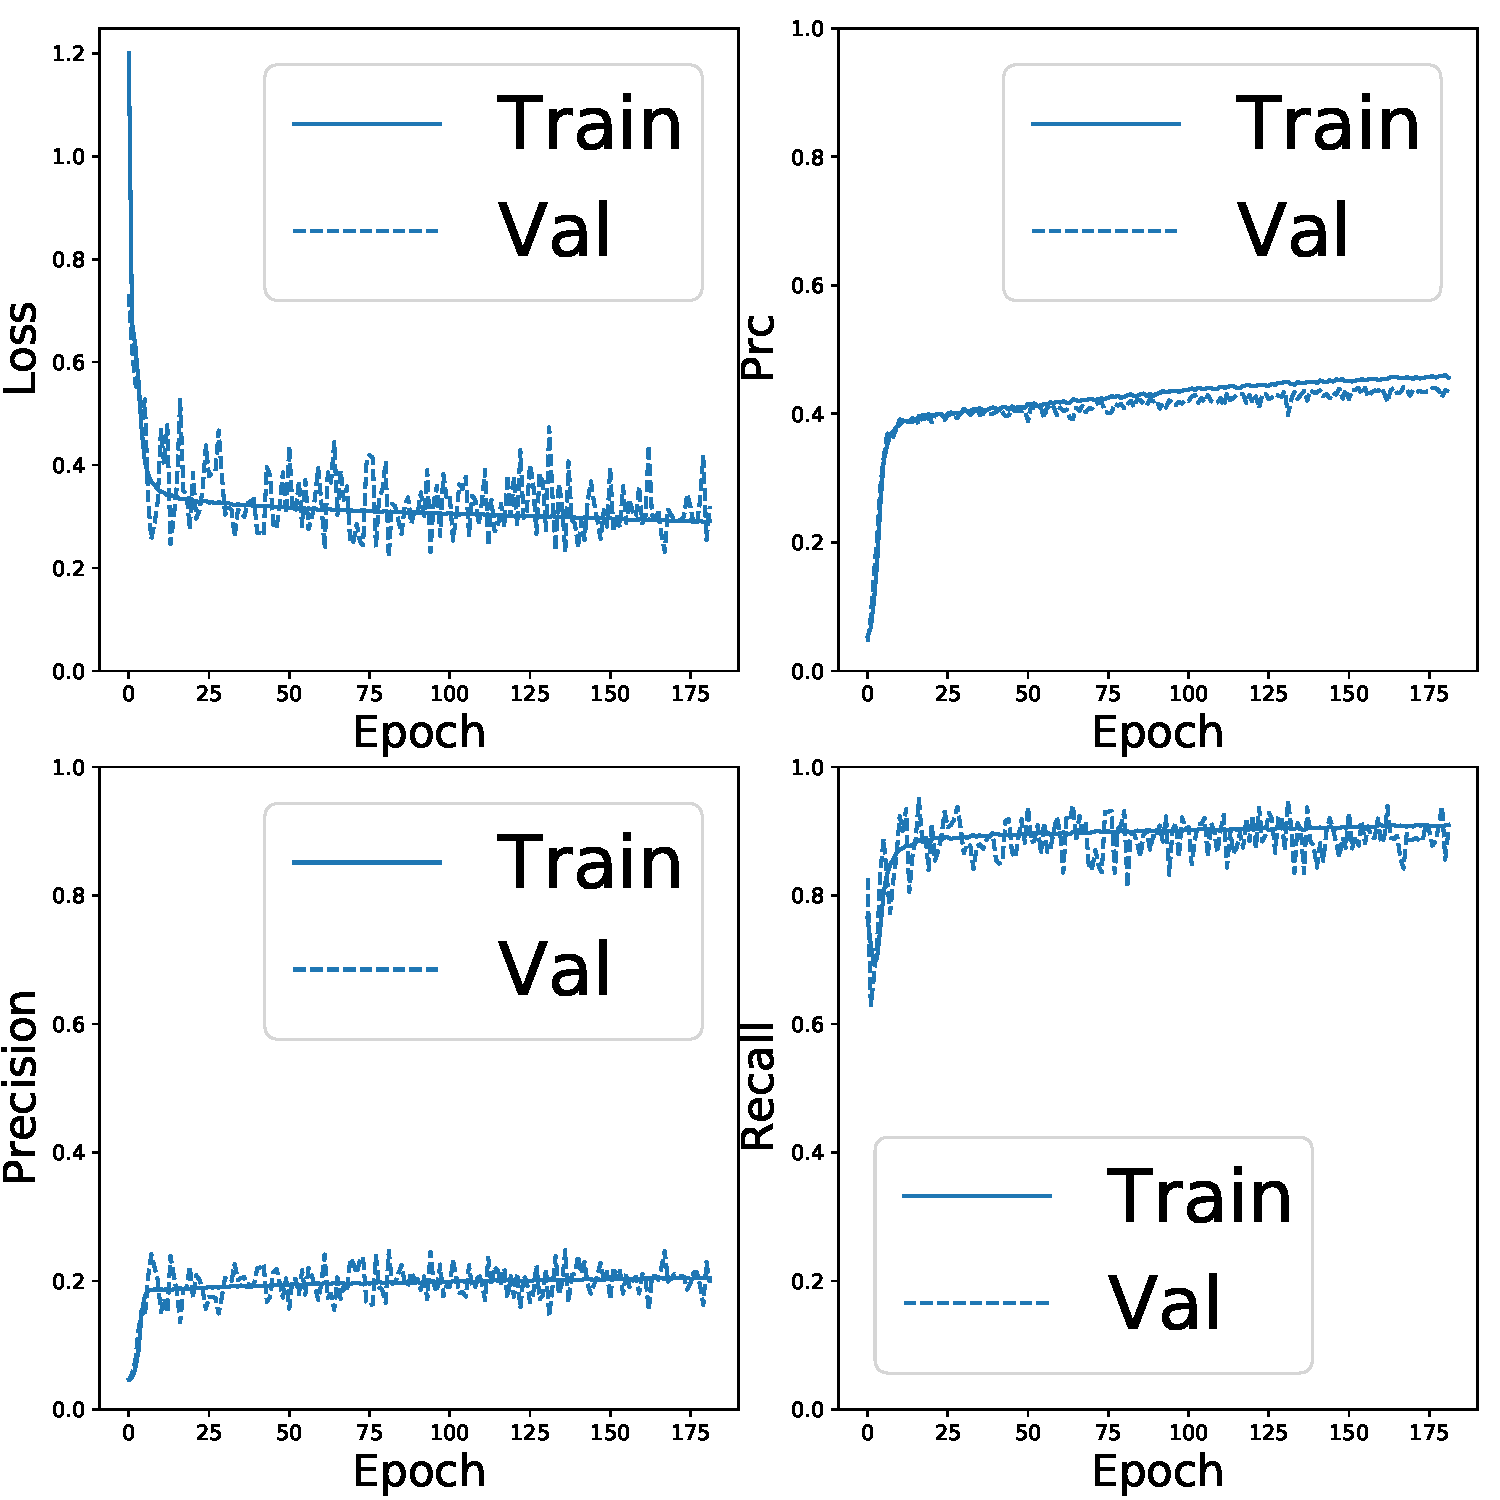
\includegraphics[scale=0.4]{Sections/HHWWgg/images/FH_DNN/BBgg/all_metrics.pdf}%
%   \caption{Metrics for Fully-Hadronic DNN bb$\gamma \gamma$ killer. Loss w.r.t. epoch(top left). Precision-Recall curve w.r.t. epoch. Precision is defined as $\frac{(TruePositive)}{(TruePositive)+(FalsePositive)}$ and recall is defined as $\frac{(TruePositive)}{(TruePositive)+(FalseNegative)}$(top right). Precision w.r.t. epoch (bottom left). Recall w.r.t. epoch (bottom right).}
%   \label{fig:FH_DNN_Metrics_bbggVsAll}
% \end{figure}

\begin{figure}[!htbp]
  \centering
  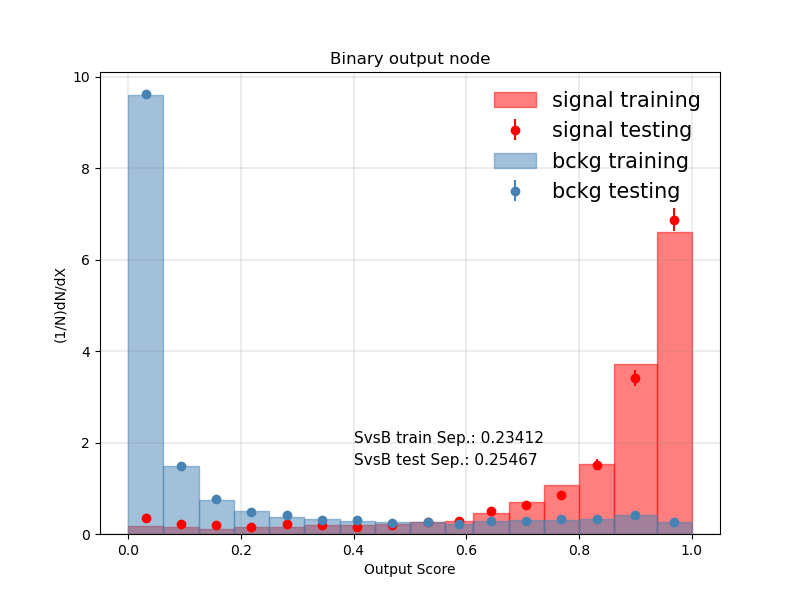
\includegraphics[scale=0.6]{Sections/HHWWgg/images/FH_DNN/BBgg/overfitting_plot_BinaryClassifier_Binary.png}%
  \caption{Output score of Fully-Hadronic DNN bb$\gamma \gamma$ killer training}
  \label{fig:FH_DNN_OutputScore_bbggVsAll}
\end{figure}

\clearpage

% @Author: Ram Krishna Sharma
% @Date:   2021-05-18
% @Last Modified by:   Ram Krishna Sharma
% @Last Modified time: 2021-05-27
\subsubsection{Categorization}
\label{subsubsec:Categorization}

Events falling into the Fully-hadronic category are categorized in a similar fasion as described in Section \ref{subsubsec:SLCategorization} for the Semi-leptonic channel, but with the addition of a selection on the bb$\gamma\gamma$ killer score. 

% The categorization is performed in a similar way as described in sec.~\ref{subsubsec:SLCategorization}, for Semi-Leptonic channel.

The expected signal region yields background processes, simulated with MC, and HH signal, both scaled to the Run 2 luminosity of 137 $fb^{-1}$ (the estimated luminosity value at the time of training), are shown in Figure \ref{fig:FH_DnnScore}
for the WW$\gamma\gamma$ identifier score.

\begin{figure}[!htbp]
  \centering
  % 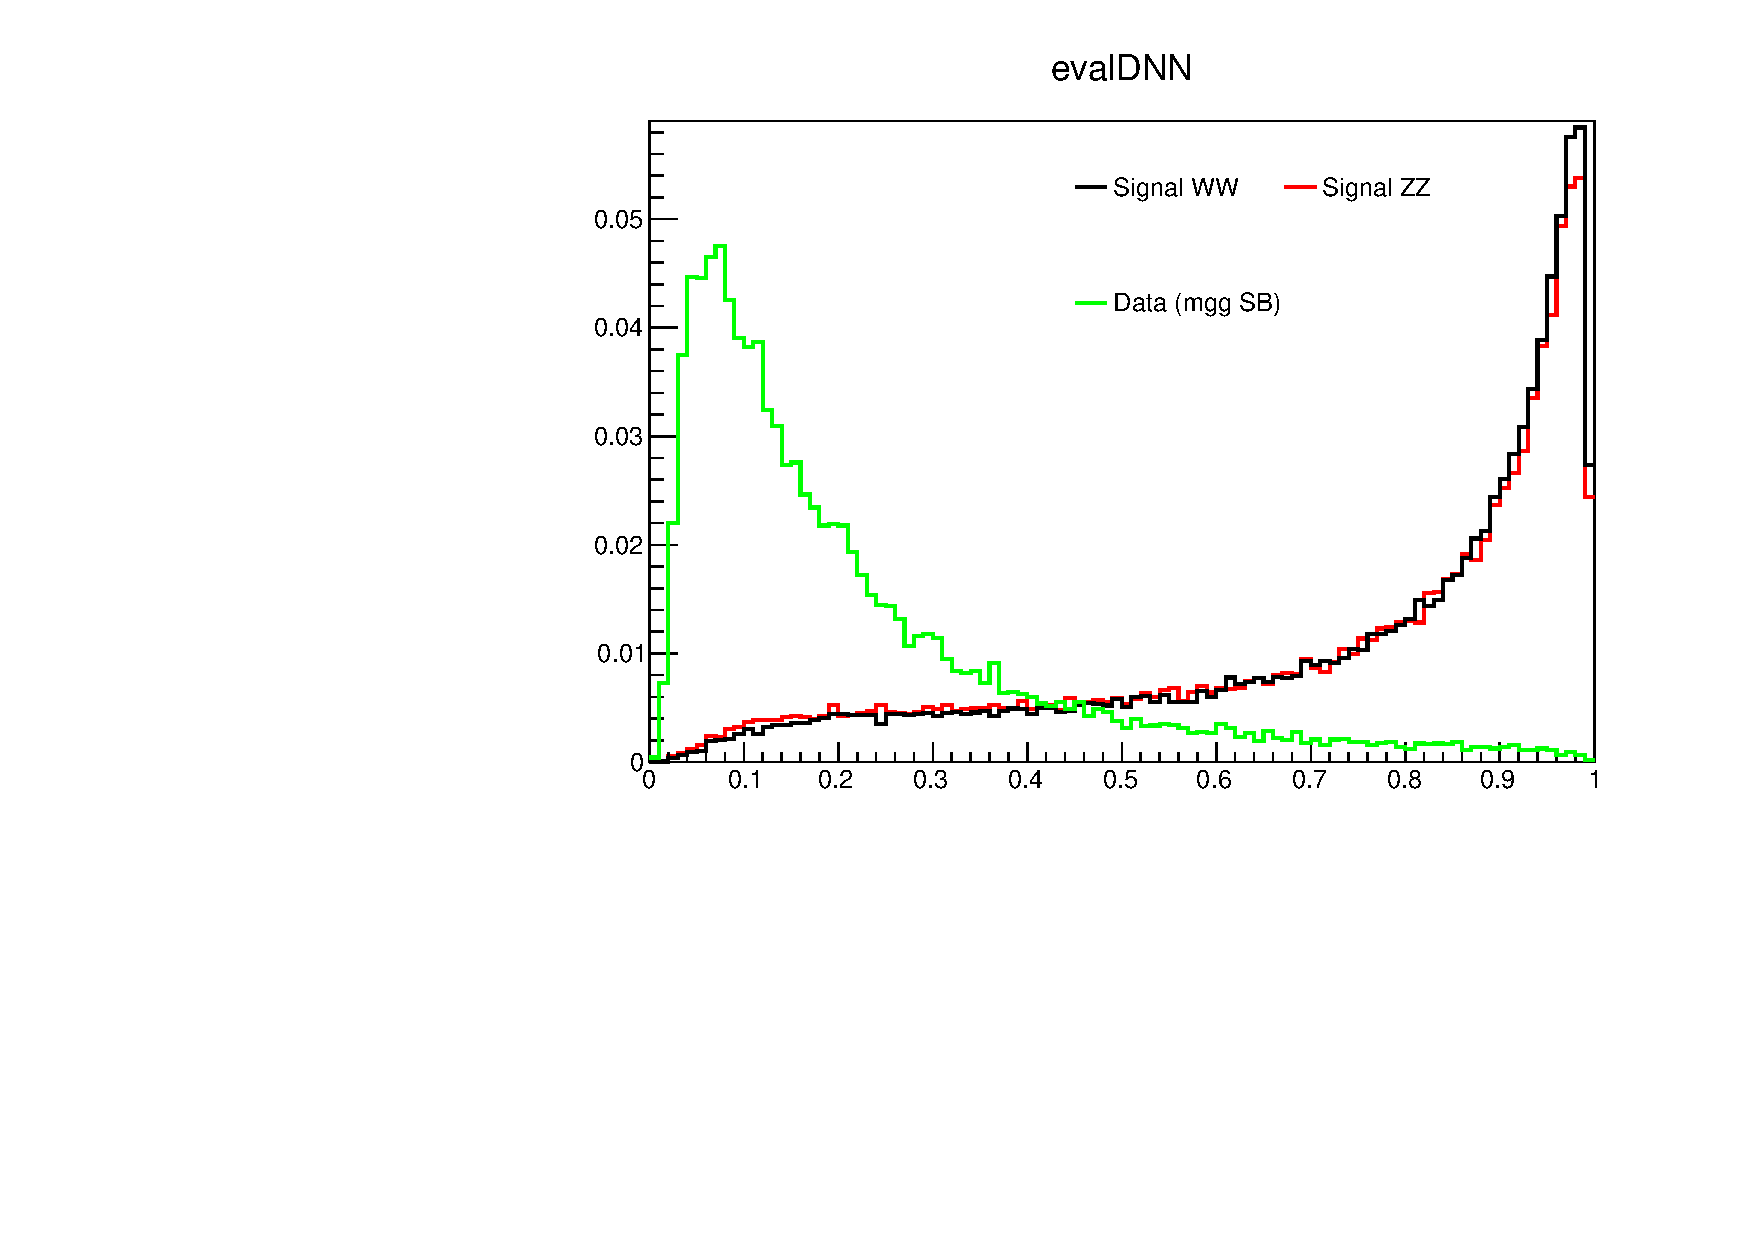
\includegraphics[scale=0.6]{Sections/HHWWgg/images/FH_DNN/evalDNN.pdf}
  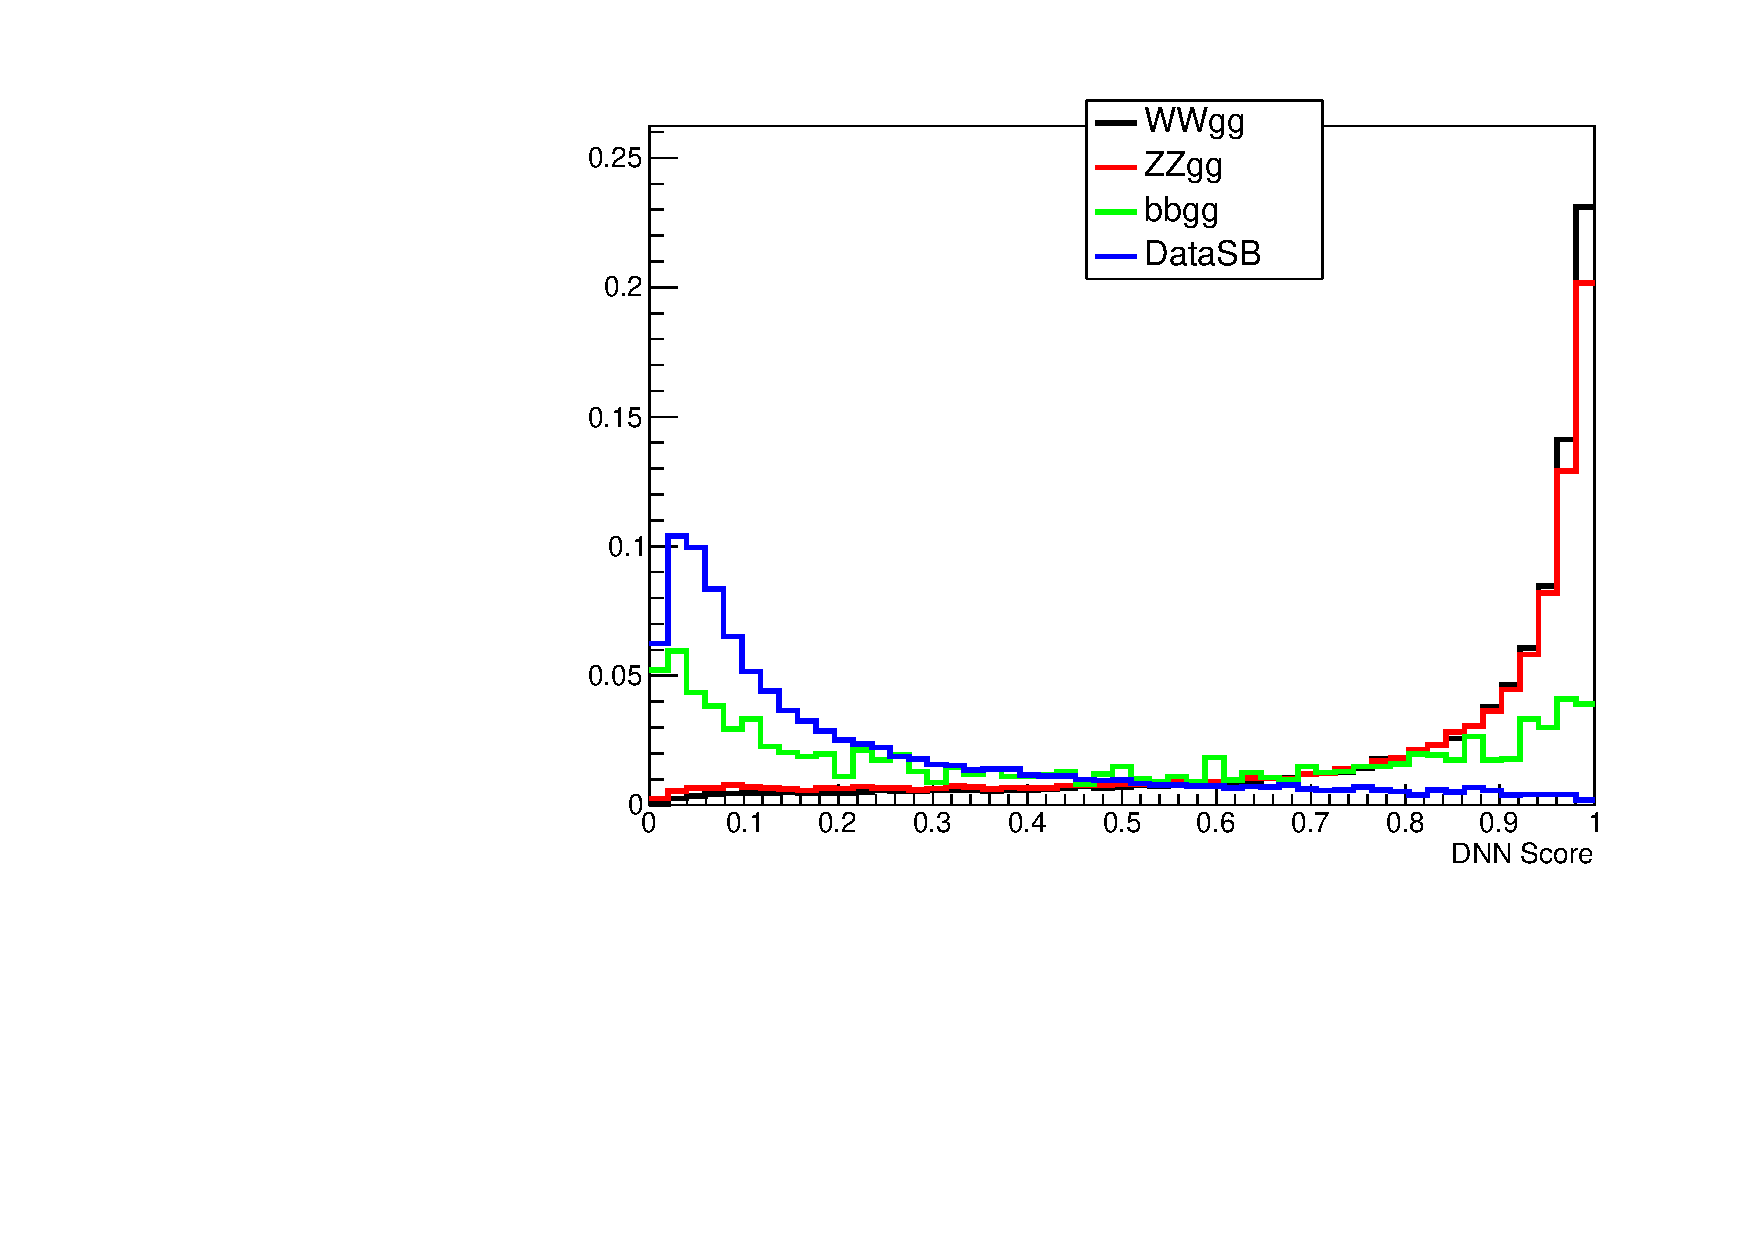
\includegraphics[scale=0.6]{Sections/HHWWgg/images/FH_DNN/WWvsAll_2017_NormUnity_BBggScoreCut0p6.pdf}
  \caption{Fully-Hadronic output score for signal and background. All distributions are normalized to unity.}
  \label{fig:FH_DnnScore}
\end{figure}

These distributions are used for significance computations. 

In performing the categorization, the same method is followed as for the semi-leptonic final state described in Section \ref{subsubsec:SLCategorization}. The result of smoothing of the MC in the signal region is shown in Fig.~\ref{fig:FH_smoothing}.

\begin{figure}[!htbp]
  \centering
  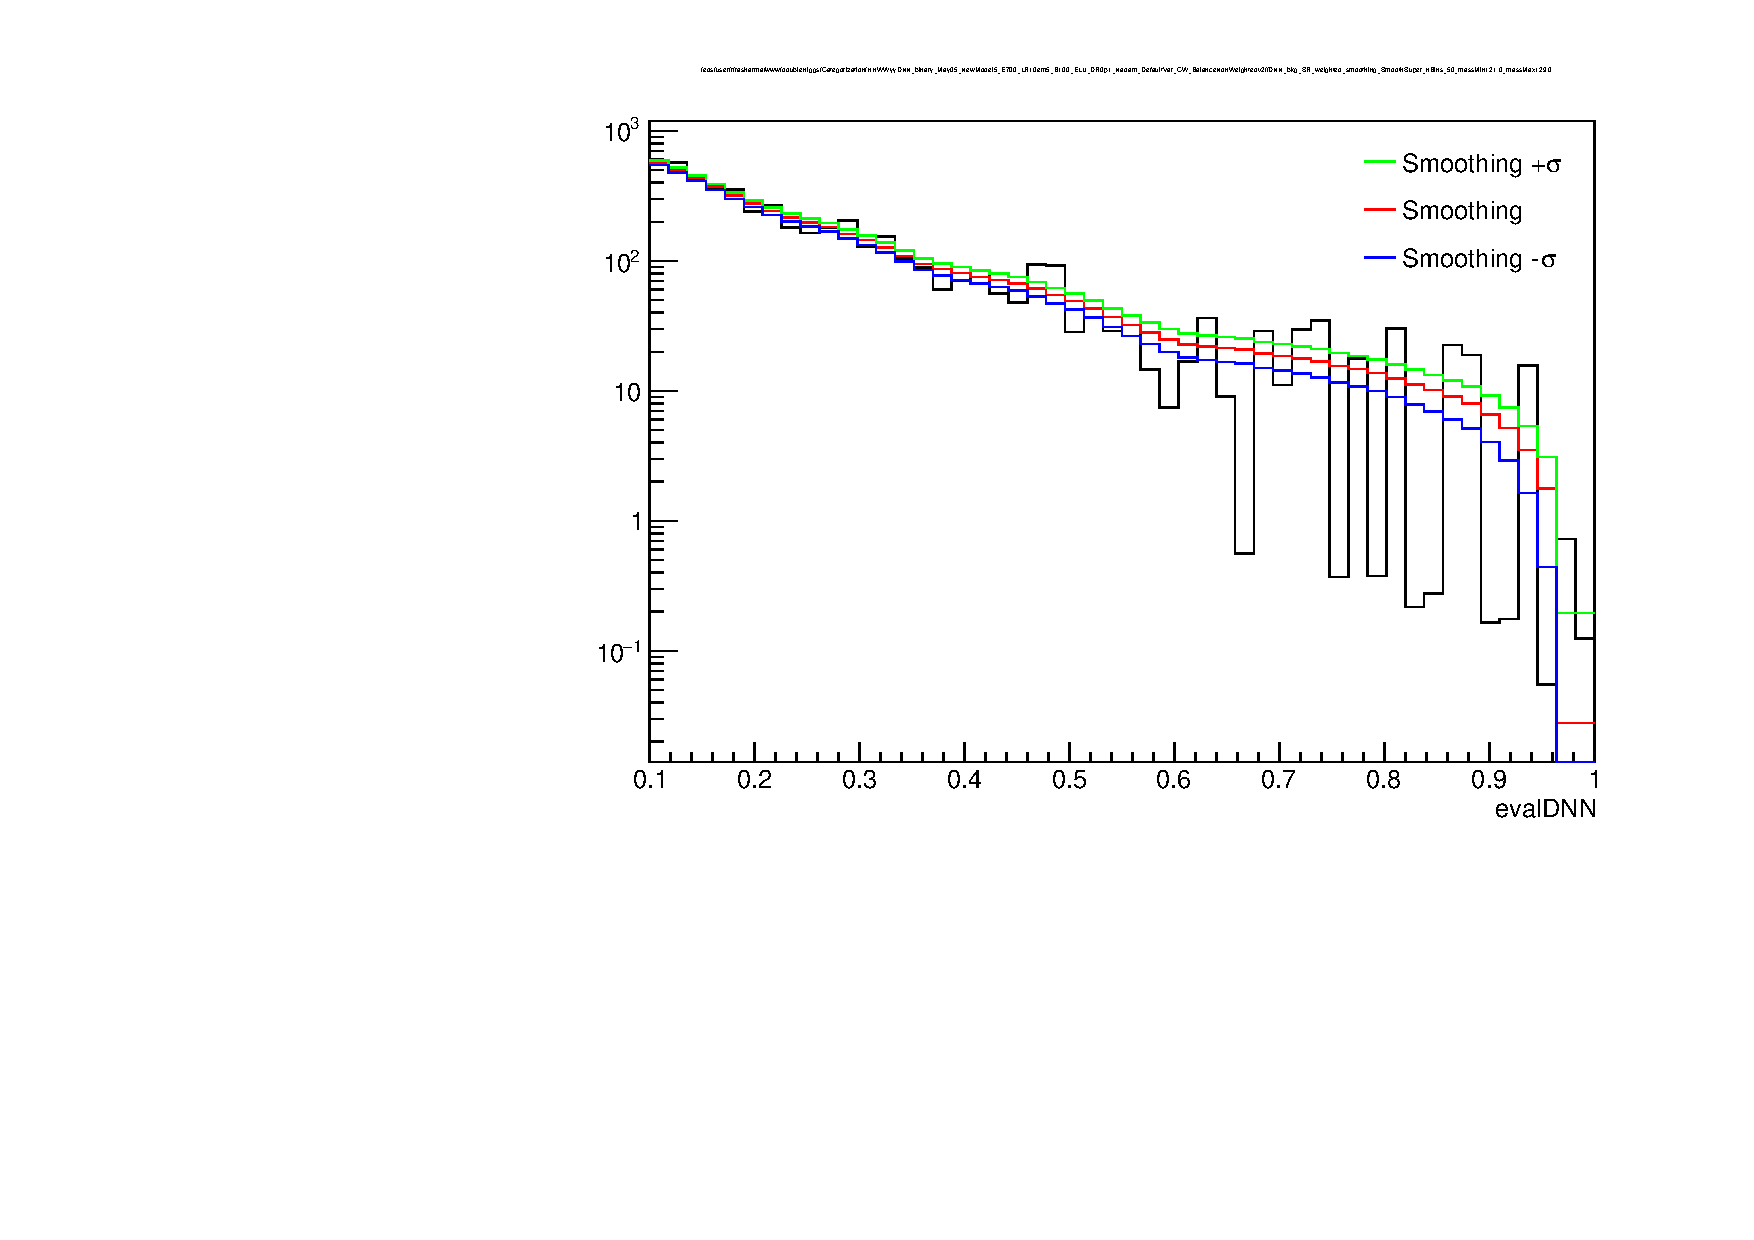
\includegraphics[scale=0.6]{Sections/HHWWgg/images/FH_DNN/h_DNN_bkg_SR_weighted_smoothing_SmoothSuper_nBins_50_massMin121_0_massMax129_0.pdf}
  \caption{Result of background smoothing for Fully-Hadronic channel.}
  \label{fig:FH_smoothing}
\end{figure}

The optimal categorization was chosen based on the 380 bin case, in which category boundaries are simultaneously optimized among 380 equally sized bins of width (1/380) from output WW$\gamma\gamma$ identifier DNN scores of 0.1 to 1.
It was also found that a signal region definition of 120 to 130 GeV in the di-photon mass region returns the greatest significance with number of bins and categories held constant,
a hint that choosing optimal category boundaries based on this definition may return the most sensitive result.
The category boundaries, yields and significance values are summarized in Tab.~\ref{tab:FHcategories_4} for the case of four categories, the final choice on number of categories for optimization.

After categorizing based on the WW$\gamma\gamma$ identifier to maximize signal efficiency, events are required to have a bb$\gamma\gamma$ killer score less than 0.6 in order to remove the majority of bb$\gamma\gamma$ events.

\begin{table}[!htbp]
  \begin{center}
    \begin{tabular}{|c|c|c|c|c|c|c|}
    \hline
    CatN & DNN Min & DNN Max & S        & $B_{SR}$   & $Data_{Sideband}$ & Significance\\ \hline \hline
    0    & 0.983   & 1.0     & 0.03373  & 0.101421   & 24.0              & 0.03373 \\
    1    & 0.969   & 0.983   & 0.04398  & 4.684672   & 55.0              & 0.02029 \\
    2    & 0.893   & 0.969   & 0.13746  & 53.51282   & 384.0             & 0.01878 \\
    3    & 0.1     & 0.893   & 0.30157  & 5979.241   & 27390.0           & 0.00390 \\
    \hline
    \end{tabular}
  \end{center}
\caption{
    Fully-Hadronic DNN Category Boundaries and yields in signal region for 4 Categories
}
\label{tab:FHcategories_4}
\end{table}


\subsubsection{Data Driven QCD and $\gamma$jet}
\label{subsubsec:QCDDataDriven}

For this final state category, a data-driven QCD$+\gamma$jet estimation is performed in a control region where one photon candidate fails the requirement of photon ID $>$ -0.7, previously used and described in \cite{Sirunyan:2020sum}.

% This is shown in Figure \ref{fig:FH_preQCDEstimation_DataMC_photonIDDescription}, as there is a large under

% in a similar manner as perfomed for the ttH analysis in \href{https://cms.cern.ch/iCMS/analysisadmin/cadilines?line=HIG-19-013&tp=an&id=2281&ancode=HIG-19-013}{HIG-19-013}~\cite{Sirunyan:2020sum}. 

% This method is described briefly here and for details please check \cite{Sirunyan:2020sum}.

% At pre-selection level, the dominant background in the Fully-Hadronic channel are QCD multijet production in assosciation with zero to two prompt photons (``QCD + X''), composing $\approx 99\%$ of the background. However, as Fig.~\ref{fig:FH_preQCDEstimation_DataMC_photonIDDescription}(a) shows, there is a large under prediction from MC. The under prediction comes primarily from the lower region of minimum photon ID MVA\footnote{The minimum value of the photon MVA score out of the two selected photons.}, where QCD and $\gamma$ + jets MC samples do not provide an accurate description of fake photons.

% \begin{figure}[H]
%   \setcounter{subfigure}{0}
%   \centering
%   \subfloat[]{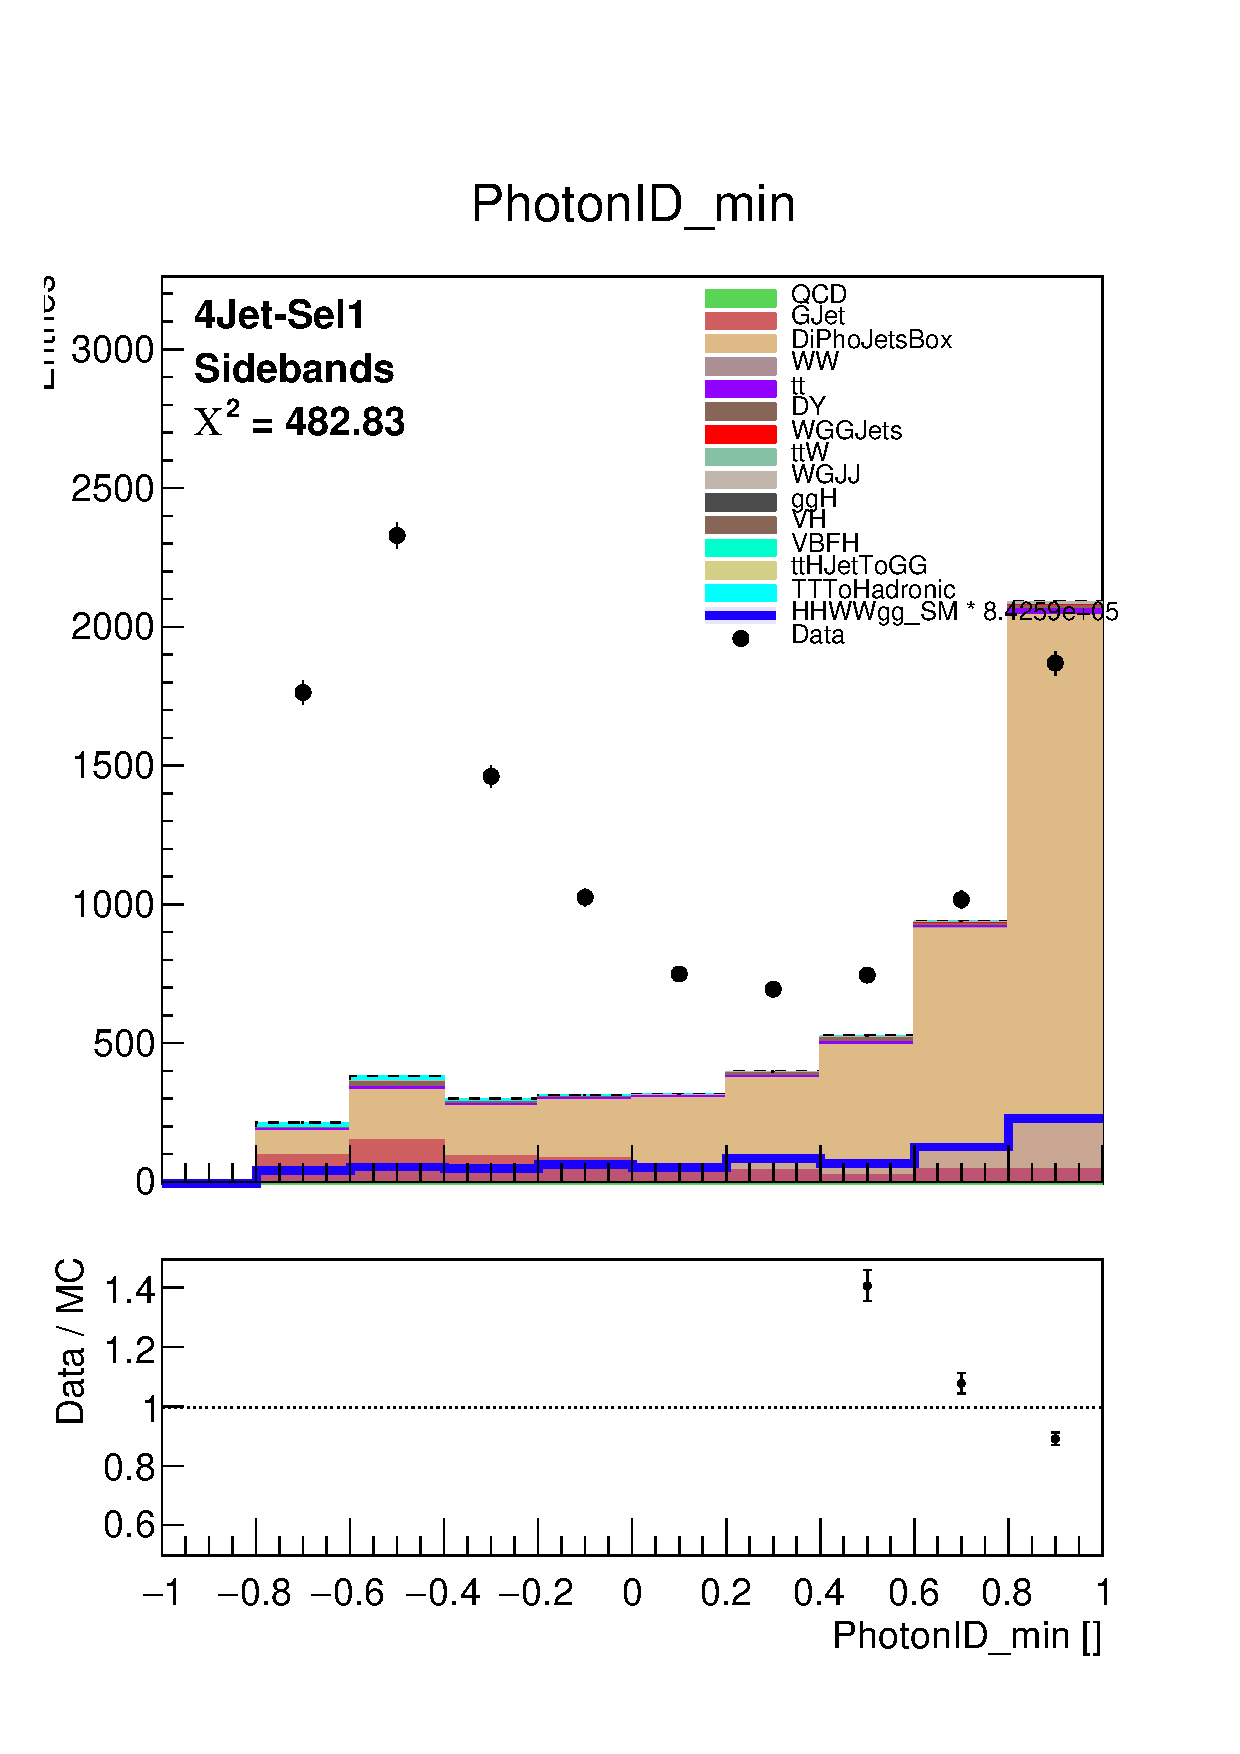
\includegraphics[width=0.45\textwidth]{Sections/HHWWgg/images/FH_DNN/DataDrivenQCD/DataMC_PhotonID_min_SB_nonLog.pdf}}
%   \qquad
%   \subfloat[]{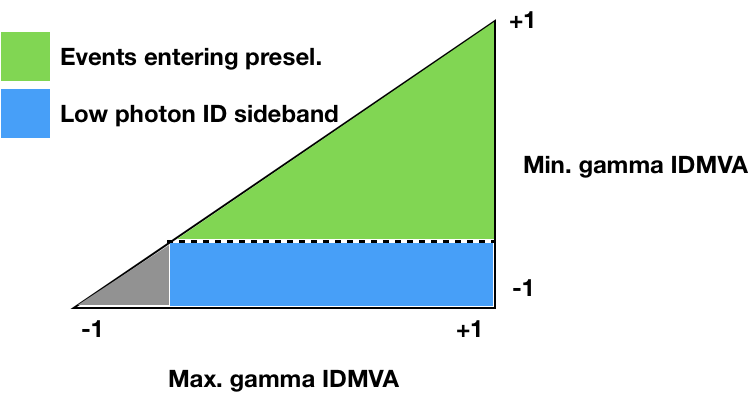
\includegraphics[width=0.45\textwidth]{Sections/HHWWgg/images/FH_DNN/DataDrivenQCD/figures_impute_photonID_diagram.png}} %%-- as of 6 Sep 2021, missing this image on gitlab 
%   \caption{(a) Minimum Photon ID MVA. (b) Diagram of the Loose MVA pre-selection (green) and the Low Photon ID Sideband (blue).}
%   \label{fig:FH_preQCDEstimation_DataMC_photonIDDescription}
% \end{figure}

% The data-driven description is obtained by using the events which fail the pre-selection cut on minimum $\gamma$ ID MVA (-0.7) in place of events from QCD and $\gamma$ + jets MC samples. This region is referred to as the ``low photon ID sideband'', as shown in Fig.~\ref{fig:FH_preQCDEstimation_DataMC_photonIDDescription}(b).

% The overall normalization of events from the low photon ID sideband should not be expected, a priori, to be the same as the number of QCD and $\gamma$+jets events in the pre-selection. To address this, a simultaneous fit in the minimum and maximum photon ID MVA is performed to obtain the scale factor. This is shown in Tab.~\ref{tab:FH_QCD_gg_SF}.
% \begin{table}[!htbp]
%     \centering
%     \begin{tabular}{|l||r|} \hline
%     Template & Scale \\ \hline
%     QCD (data driven) & 0.9 \\ \hline
%     $\gamma \gamma $+jets & 1.25 \\ \hline
%     \end{tabular}
%     \caption{Scale factor obtained from a simultaneous fit of data to MC of the minimum photon ID and maximum photon ID distributions}
%     \label{tab:FH_QCD_gg_SF}
% \end{table}

% To check our estimated background, the QCD and $\gamma$+jets MC was replaced with the data-driven background using appropriate SF given in Tab.~\ref{tab:FH_QCD_gg_SF}, the data/MC comparison was performed and shown in Fig.~\ref{fig:FH_DataMC_1}
% , ~\ref{fig:FH_DataMC_2}, ~\ref{fig:FH_DataMC_3}, and ~\ref{fig:FH_DataMC_4}. This shows that the data/mc comparison improved a lot after this estimation.
% \input{Sections/HHWWgg/sections/FH_EFT}

